\documentclass{beamer}

\usetheme{McMaster}
\usepackage{math}

%===Specific for this talk===%
\usepackage{algorithm,algorithmicx,algpseudocode}
\DeclareMathOperator{\iaa}{IAA} % paper specific
\newtheorem{proposition}{Proposition}
\newcommand{\vecw}{\left ( \vec{w}_i^n \right )^\top}
\newcommand{\Aij}{\left ( \hat{A} + E_{i \to j}^{n} \right )^{-1}}
\newcommand{\AijE}{\Aij E_{i \to j}^{n}}
\DeclareMathOperator{\Span}{span}
\DeclareMathOperator{\argmin}{argmin}
\usepackage{tikz}
\usetikzlibrary{decorations.pathreplacing,positioning,calc,intersections,3d,shapes.geometric,shapes,chains,math,fit,backgrounds}
\tikzset{
	pics/starred/.style={code={
		\filldraw[magenta] (0,0) -- (0,1) -- (1,1) -- (1,0) -- cycle;
		\filldraw[black, opacity=0.2] (0,1) -- (1,0) -- (0,0) -- cycle;
		\filldraw[black, opacity=0.4] (0,0) -- (1,1) -- (0,1) -- cycle;
%		\filldraw[red] (0,0) -- (0.5,0.5) -- (0,1) -- cycle;
%		\filldraw[blue] (0,1) -- (0.5,0.5) -- (1,1) -- cycle;
%		\filldraw[green] (1,1) -- (0.5,0.5) -- (1,0) -- cycle;
%		\filldraw[yellow] (1,0) -- (0.5,0.5) -- (0,0) -- cycle;
%		\filldraw[black, opacity=0.3] (1,0) -- (1,1) -- (0.5,1) -- (0.5,0) -- cycle;
%		\node[star, fill=magenta!30!black] at (0.5,0.5) {};
	}}
}

\title{Adaptive optimized Schwarz methods}
\author{Conor McCoid}
\institute{McMaster University \\ Joint work with Felix Kwok at the Université Laval}
\date{January 24th, 2025}

\renewcommand*{\thefootnote}{\fnsymbol{footnote}}

\begin{document}

\maketitle

\begin{frame}{Outline}

\begin{enumerate}
\item Introduction to domain decomposition
\item Adaptive optimized Schwarz methods
	\begin{enumerate}
	\item Condensed form of the iteration
	\item Iterative action approximation
	\item Adaptive transmission conditions
	\end{enumerate}
\item Numerical results
\item Future work
\end{enumerate}
\end{frame}

\section{Introduction to domain decomposition} % 15 min

% Schwarz (incl. keyhole domain)
\begin{frame}{H.A. Schwarz, 1869}

How do we solve the Laplace equation on complicated domains?

We split the domain into simpler subdomains.

\begin{figure}
	\centering
	\begin{tikzpicture}
		\begin{scope}[blend group = soft light]
			\filldraw[draw=black, fill=red!50!white, thick] (0,0) circle (1.5);
			\filldraw[draw=black, fill=green!50!white, thick] (0,-1) rectangle (3,1);
		\end{scope}
		\node[left] at (-1.5,0) {$\Omega_1$};
		\node[right] at (3,0) {$\Omega_2$};
		\node[left] at (0,0) {$\Gamma_2$};
		\node[right] at (1.5,0) {$\Gamma_1$};
	\end{tikzpicture}
%\vspace{-3em}
%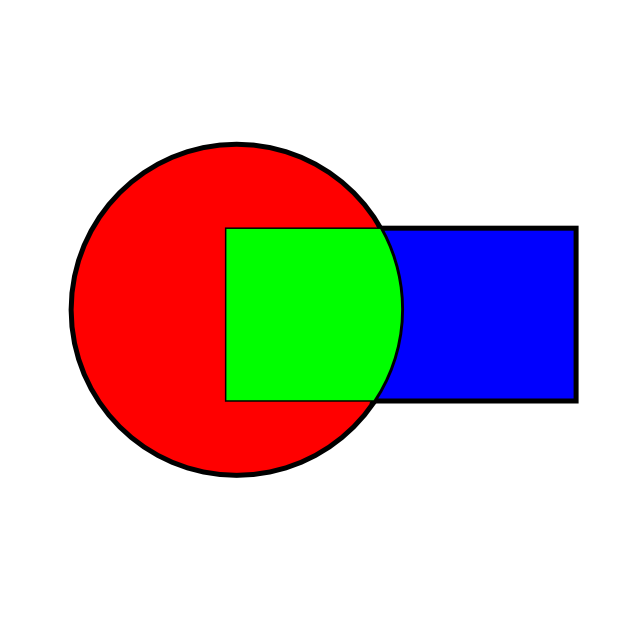
\includegraphics[width=0.5\textwidth]{AOSM/FIG_keyhole.png}
%\vspace{-4em}
%\caption{Schwarz's original example, taken from wikimedia.org}
\end{figure}

Alternating Schwarz method:
\begin{equation*}
	\begin{cases} \Delta u_1^{n+1} = 0 & \text{in } \Omega_1, \\ u_1^{n+1} = u_2^n & \text{on } \Gamma_1, \end{cases}
	\quad
	\begin{cases} \Delta u_2^{n+1} = 0 & \text{in } \Omega_2, \\ u_2^{n+1} = u_1^{n+1} & \text{on } \Gamma_2. \end{cases}
\end{equation*}
\end{frame}

\begin{frame}{Simple example}

\begin{equation*}
	u''(x) = -1, \quad x \in [-1,1], \quad u(-1)=u(1) = 0
\end{equation*}
\begin{equation*}
	\Omega_1 = [-1,0.18], \quad \Omega_2 = [-0.22, 1]
\end{equation*}

\begin{figure}
	\only<1>{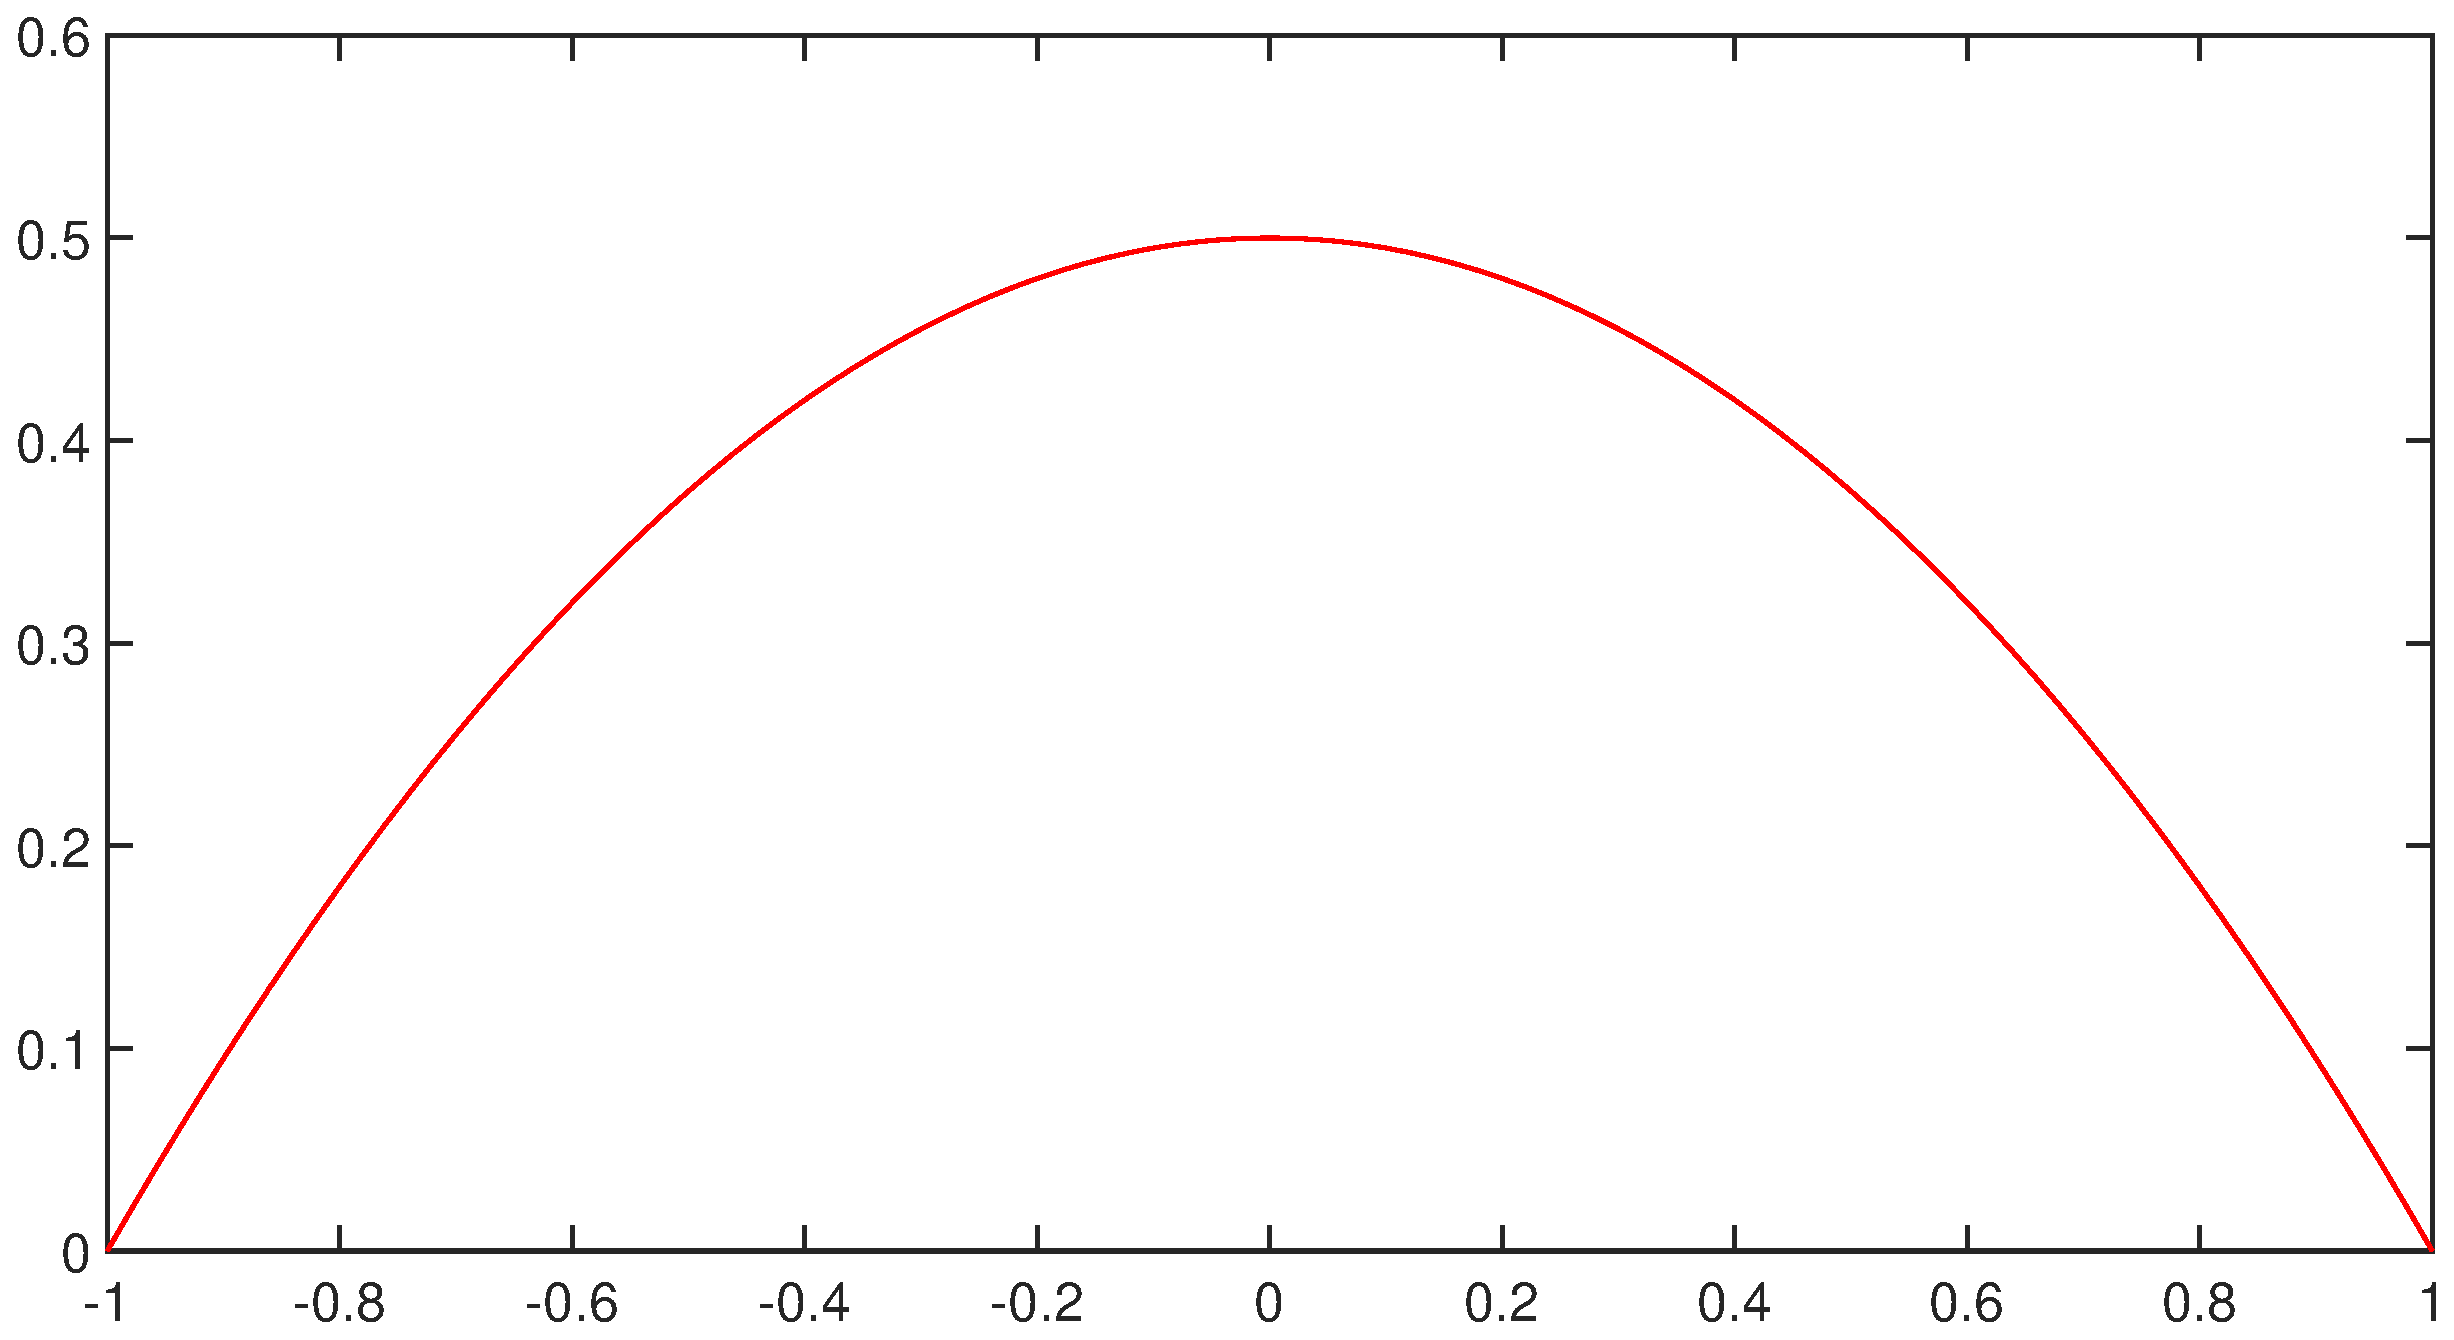
\includegraphics[width=\textwidth]{AOSM/PLOT_SimpleSchwarz1.eps}}
	\only<2>{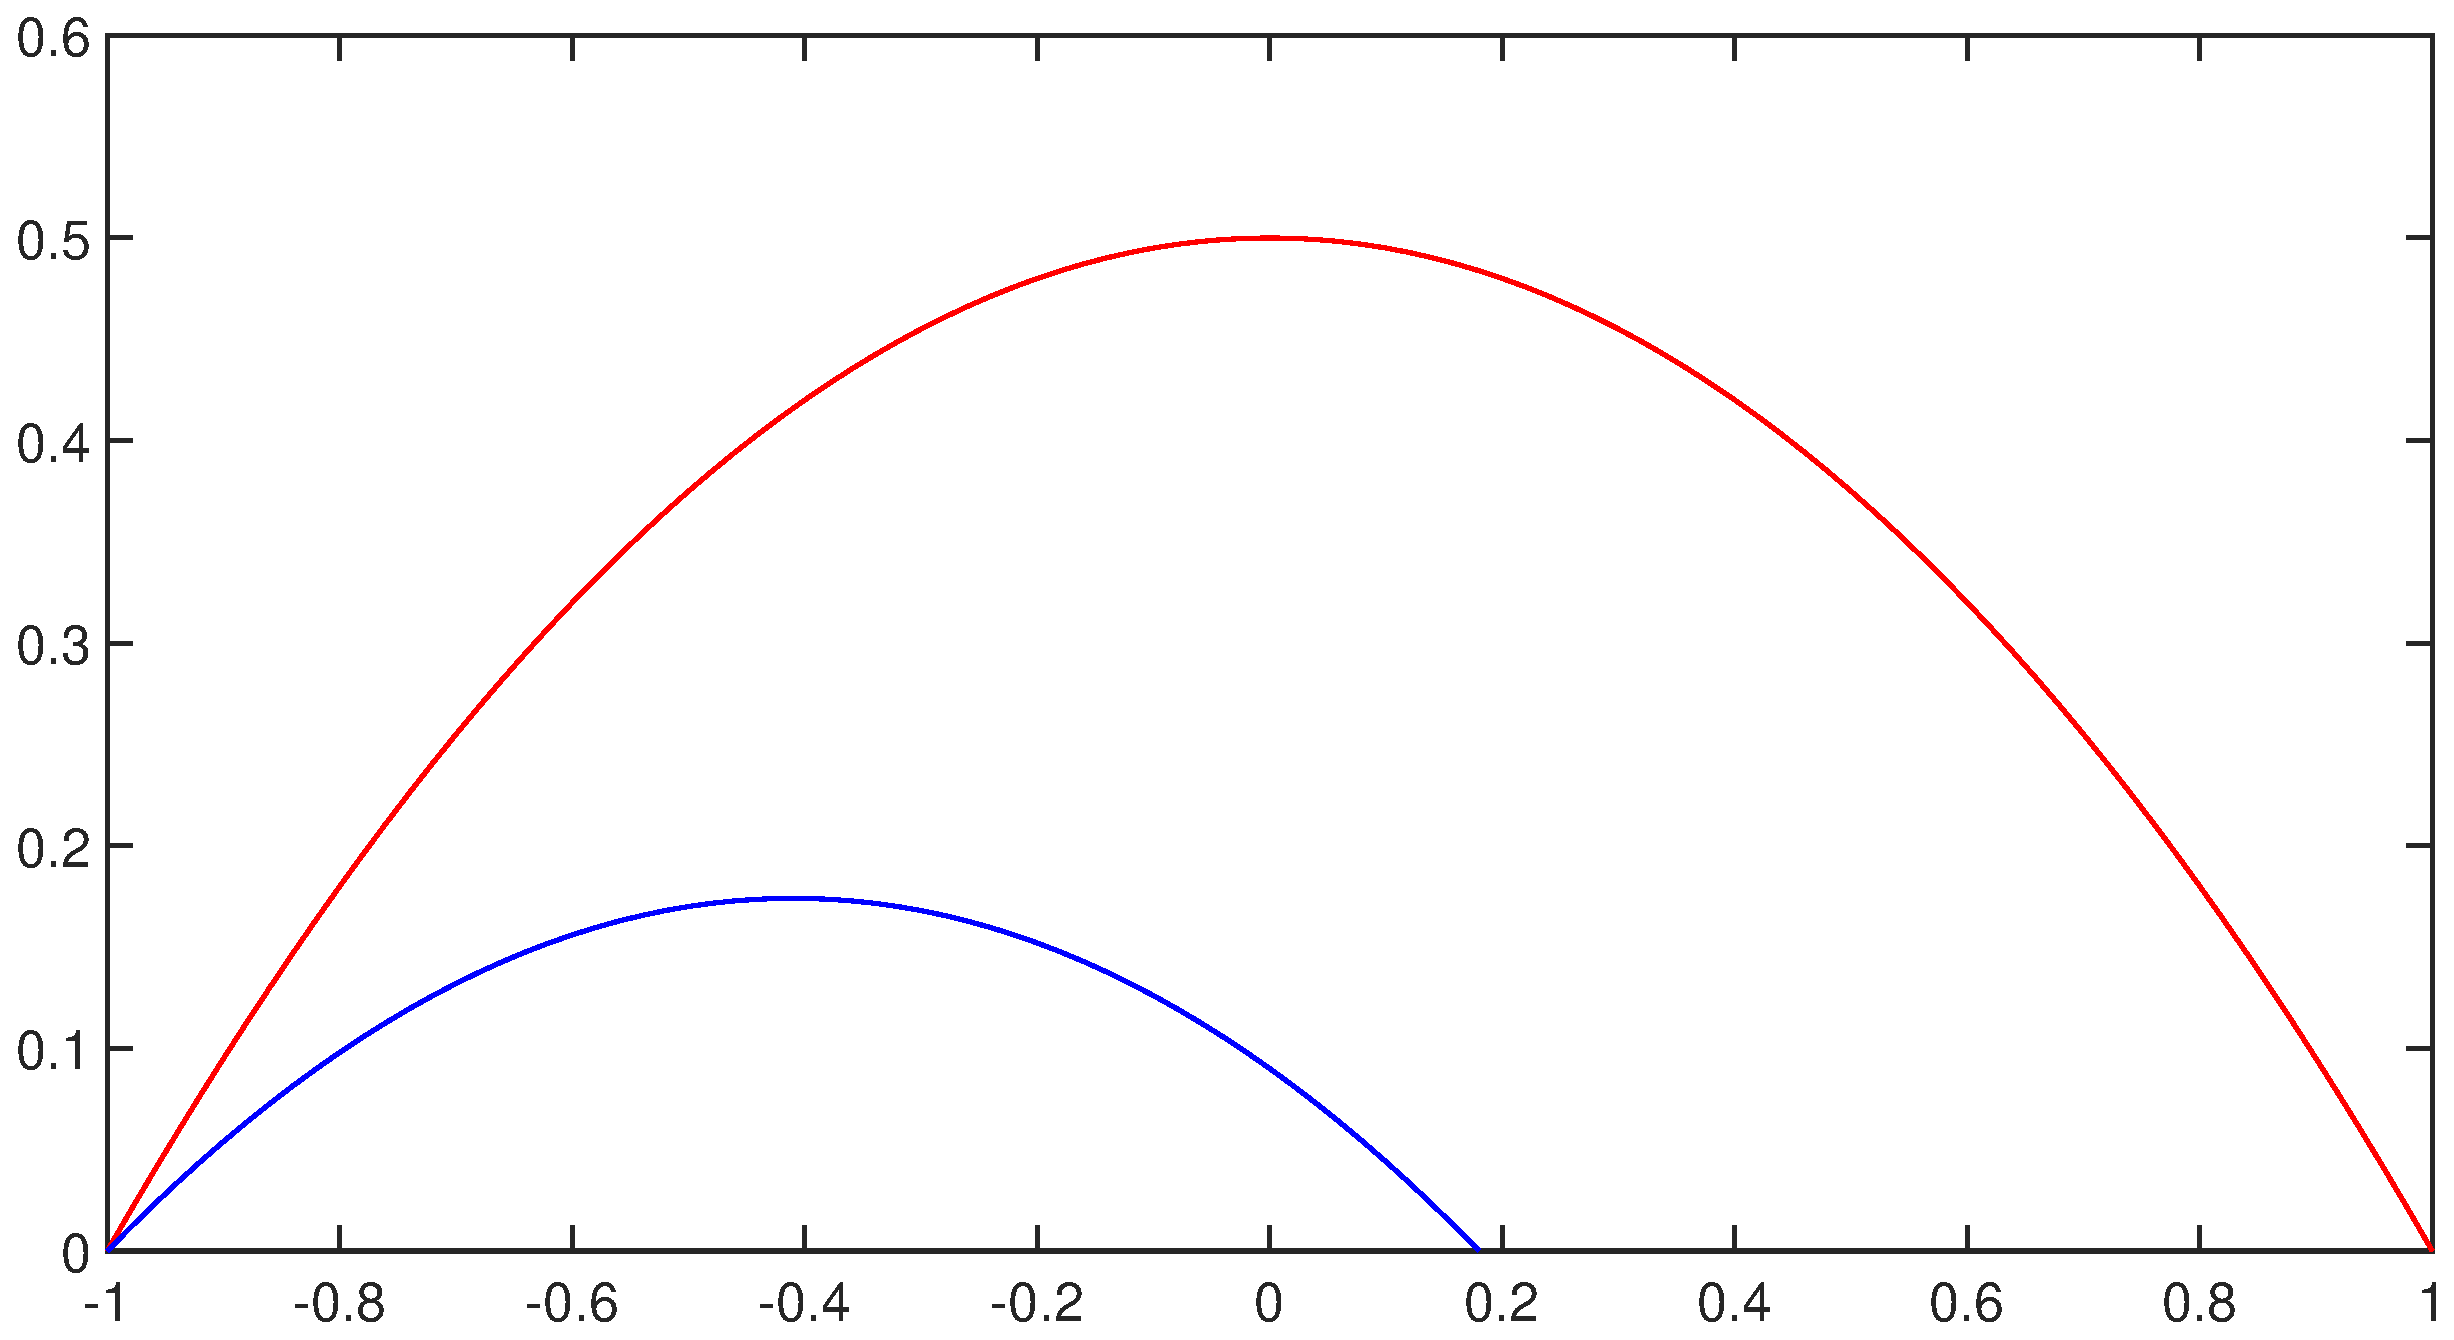
\includegraphics[width=\textwidth]{AOSM/PLOT_SimpleSchwarz2.eps}}
	\only<3>{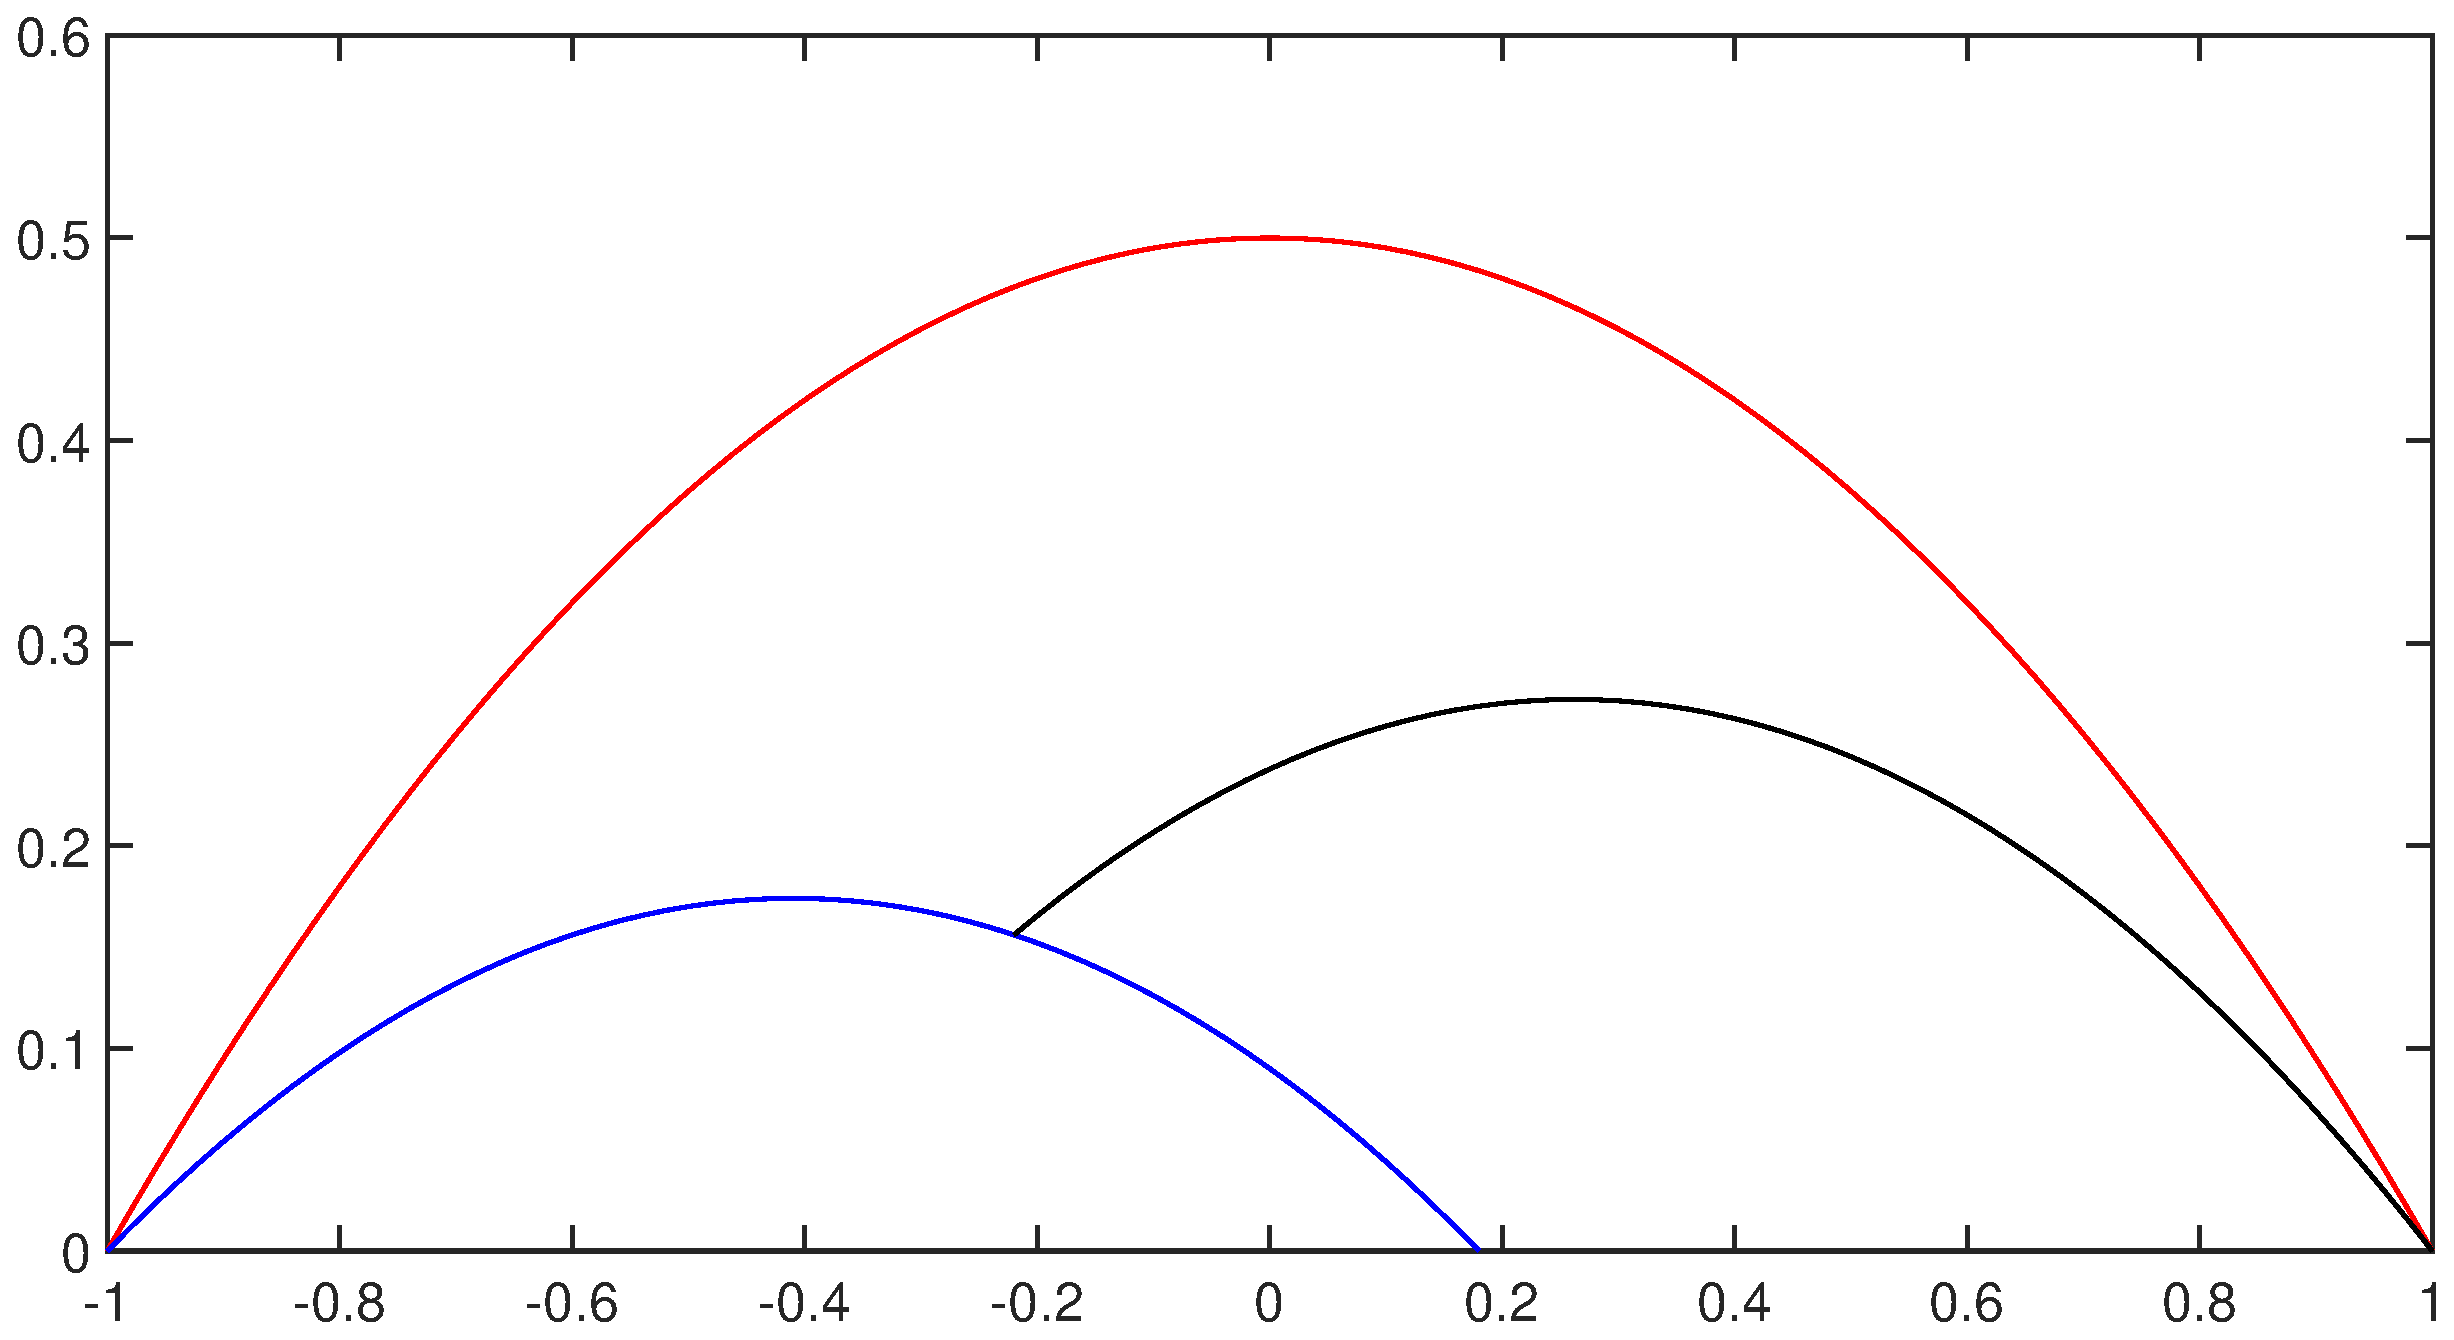
\includegraphics[width=\textwidth]{AOSM/PLOT_SimpleSchwarz3.eps}}
	\only<4>{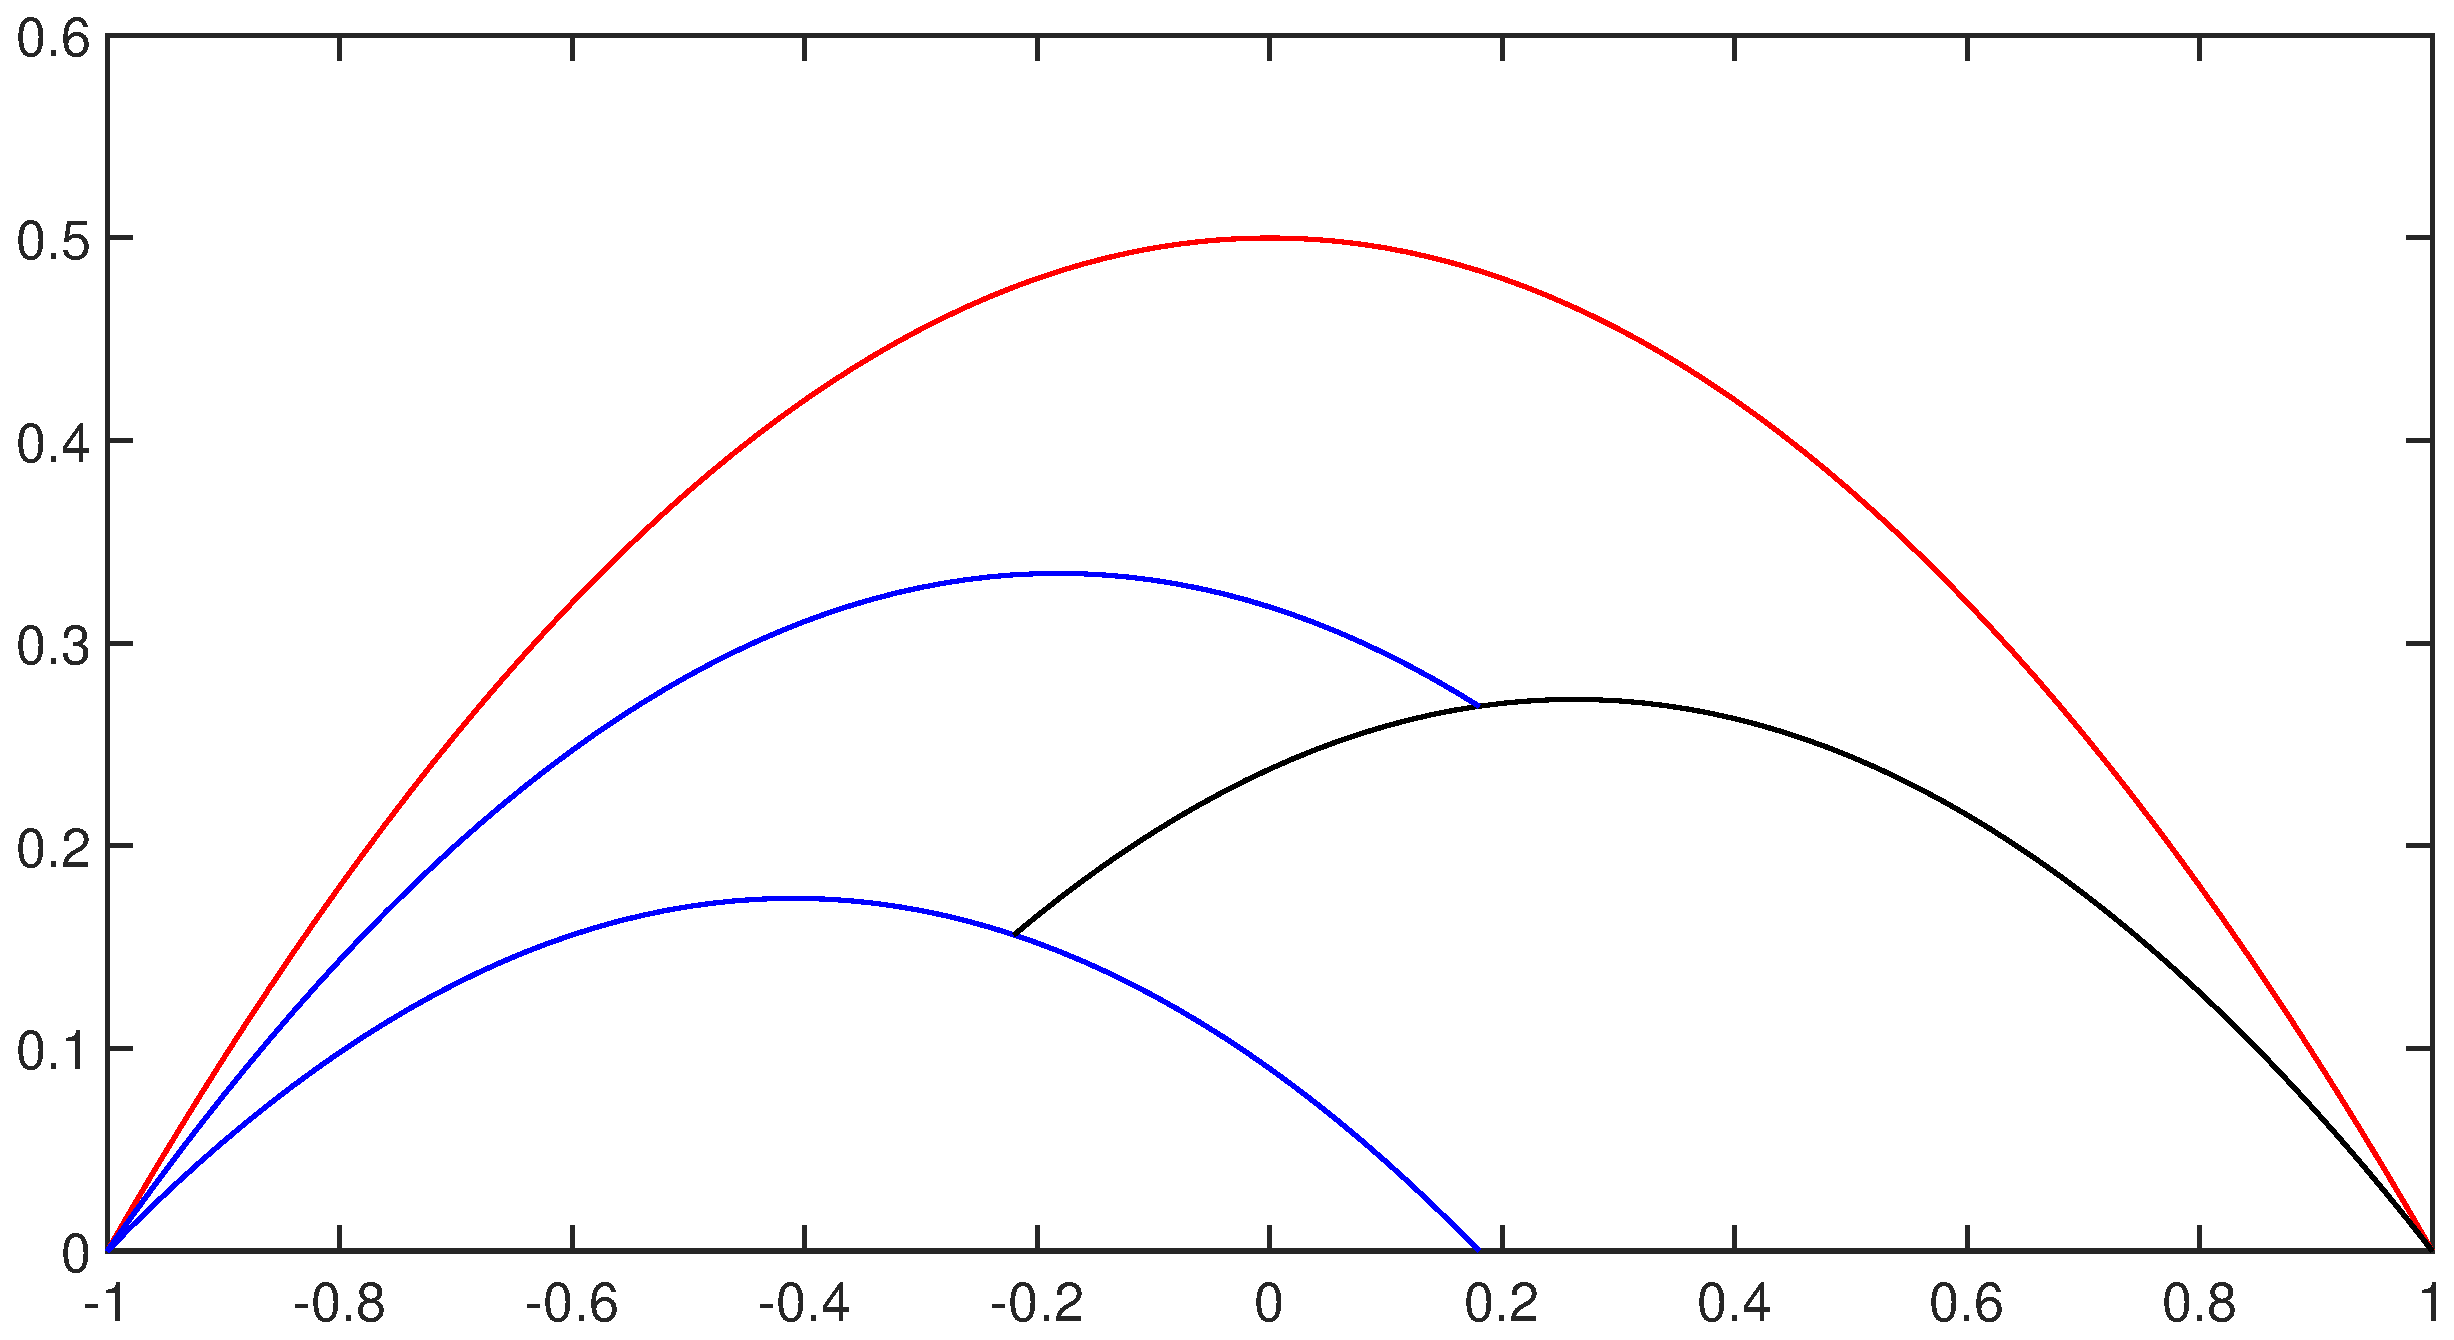
\includegraphics[width=\textwidth]{AOSM/PLOT_SimpleSchwarz4.eps}}
	\only<5>{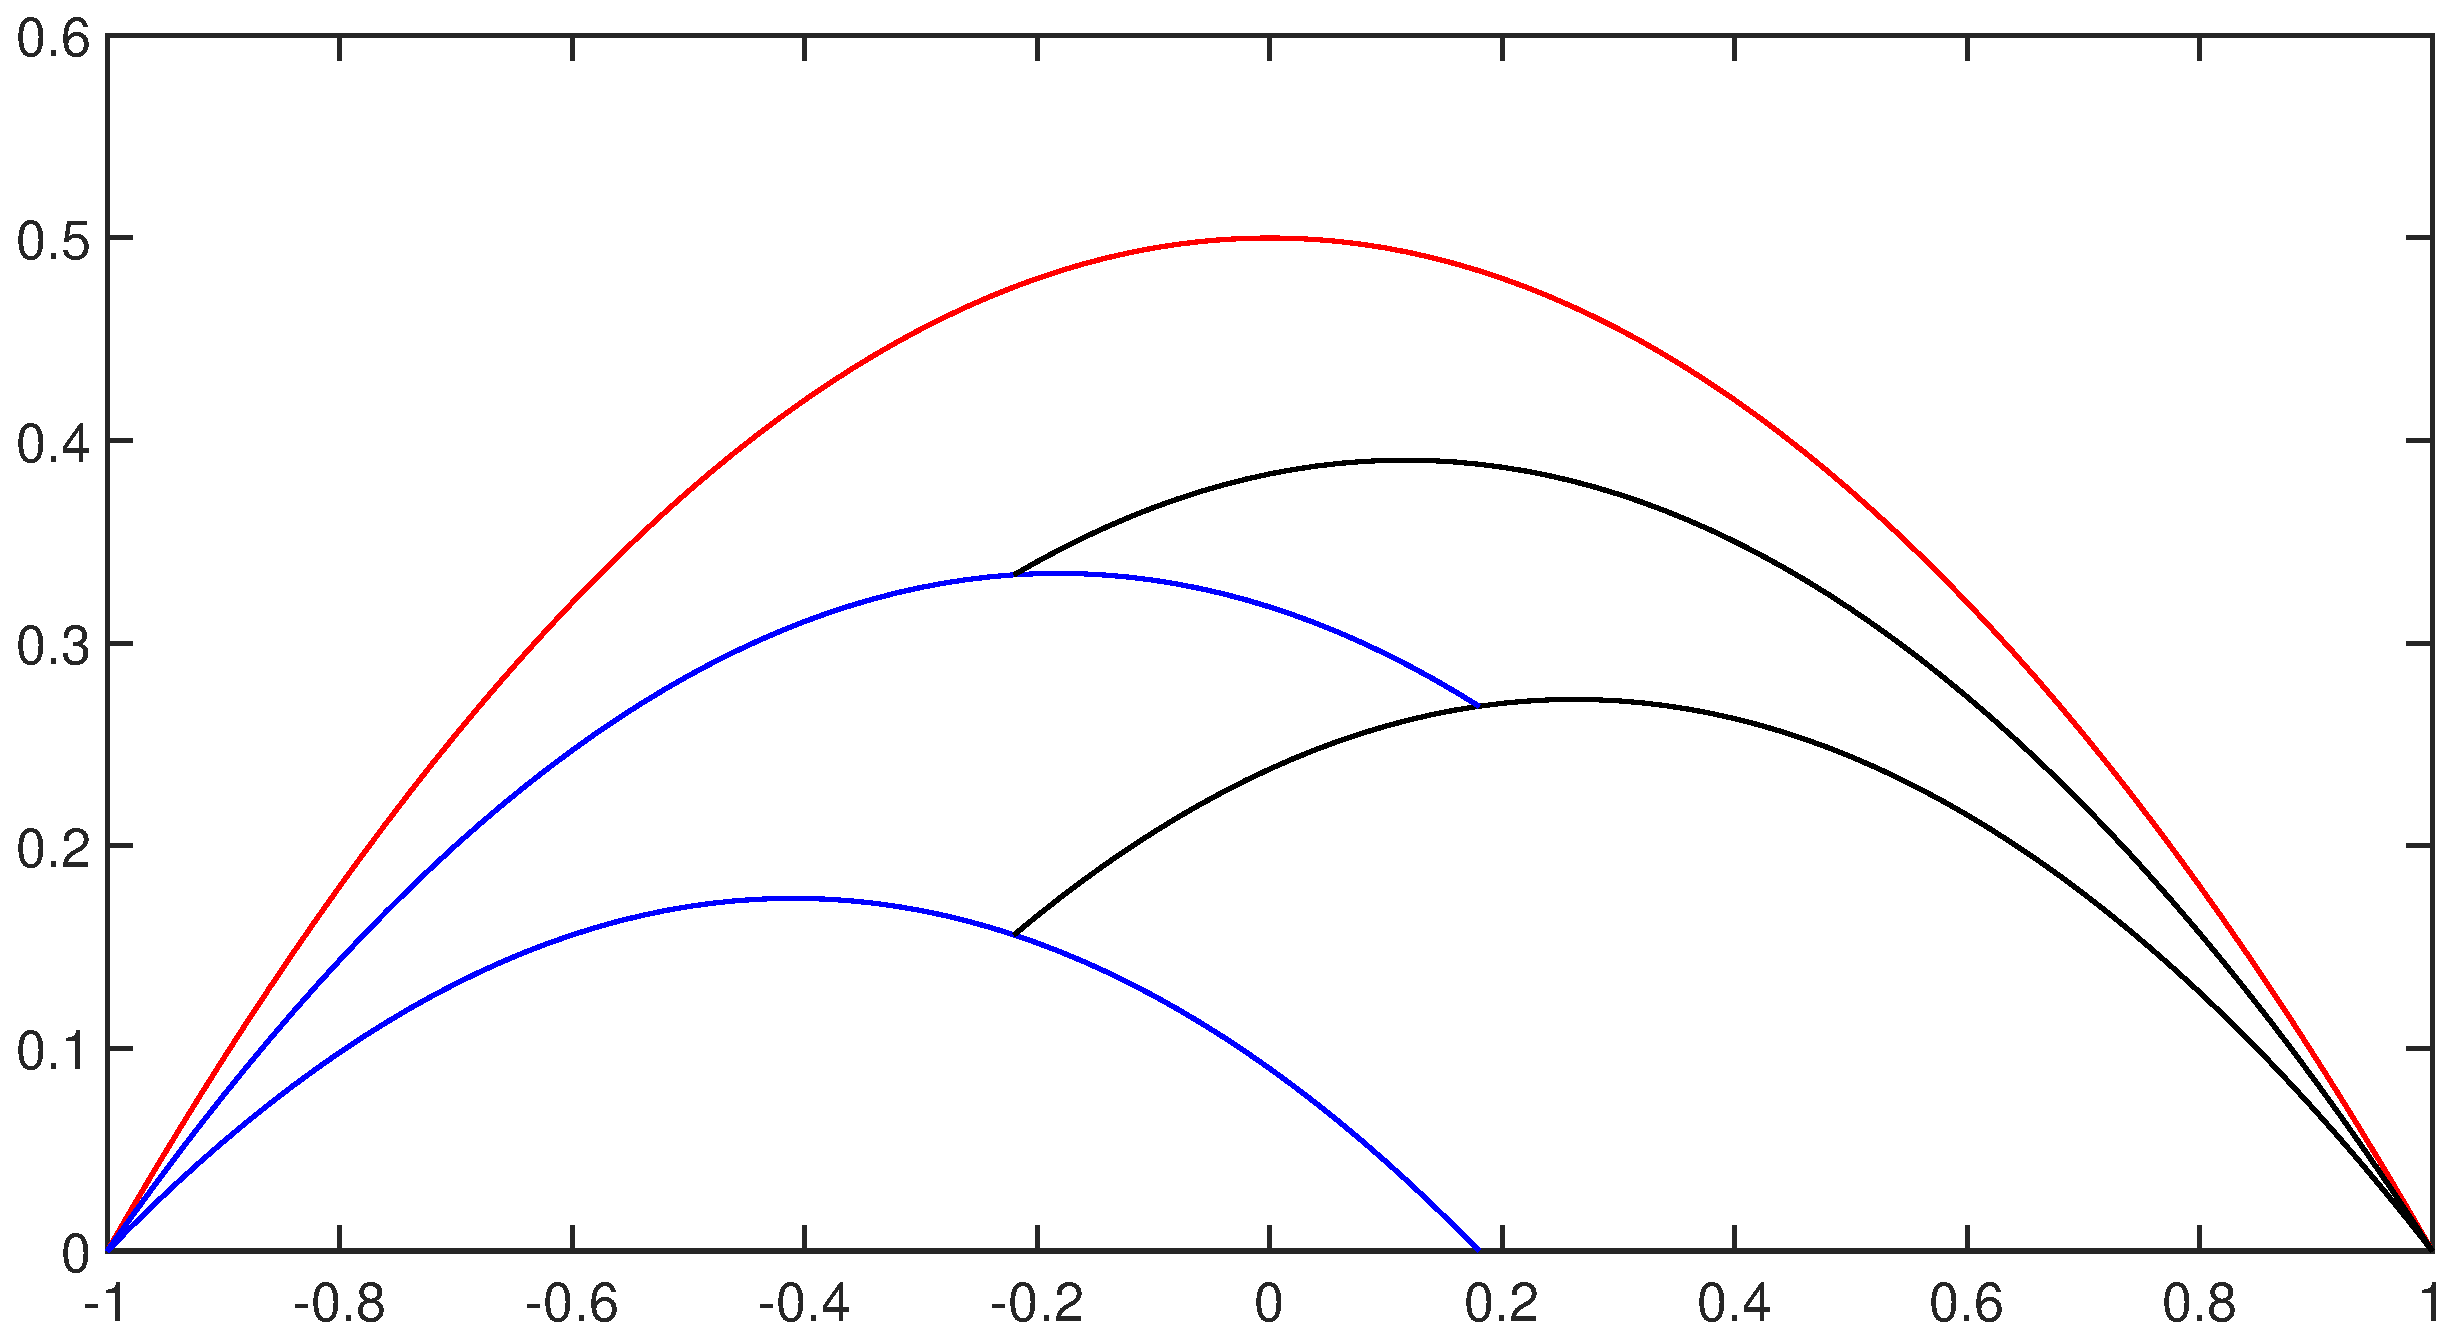
\includegraphics[width=\textwidth]{AOSM/PLOT_SimpleSchwarz5.eps}}
\end{figure}
\end{frame}

%% P.L. Lions
%\begin{frame}{P.L. Lions, 1989}
%
%Parallel Schwarz method:
%\begin{equation*}
%	\begin{cases} \Delta u_1^{n+1} = 0 & \text{in } \Omega_1, \\ u_1^{n+1} = u_2^n & \text{on } \Gamma_1, \end{cases}
%	\quad
%	\begin{cases} \Delta u_2^{n+1} = 0 & \text{in } \Omega_2, \\ u_2^{n+1} = u_1^{n} & \text{on } \Gamma_2. \end{cases}
%\end{equation*}
%
%Multiple subdomains:
%\begin{equation*}
%	\begin{cases} \Delta u_i^{n+1} = 0 & \text{in } \Omega_i, \\ u_i^{n+1} = u_j^n & \text{on } \Gamma_{ij} \end{cases}
%\end{equation*}
%where $\Gamma_{ij}$ is the boundary of $\Omega_i$ that lies in $\Omega_j$.
%\end{frame}

\begin{frame}{Discretization of continuous problem}

Suppose we have an elliptic PDE:
\begin{equation*}
	\begin{cases} \Delta u(x,y) = f(x,y), & x,y \in \Omega, \\ u(x,y) = g(x,y), & x,y \in \partial \Omega, \end{cases}
\end{equation*}
that we solve with finite differences on a structured grid:
\begin{align*}
	\Delta u_{i,j}
	\approx \frac{ u_{i+1,j} + u_{i-1,j} + u_{i,j+1} + u_{i,j-1} - 4u_{i,j} }{h^2}.
\end{align*}

\begin{figure}
	\begin{tikzpicture}[scale=0.8]
		\draw[step=1em,black] (0,0) grid (10em,10em);
		\node[above] at (5em,10em) {$\Omega$};
	\end{tikzpicture}
\end{figure}
\end{frame}

\begin{frame}{Domain decomposition}

We split the domain into two along a line $x=x_\Gamma$.
This gives us two domains $\Omega_1$ and $\Omega_2$, as well as the interface between them, $\Gamma$.

\begin{figure}
	\begin{tikzpicture}
		\matrix[row sep=1em, column sep=1em, ampersand replacement=\&]{
%			\draw[step=1em,black] (0,0) grid (10em,10em);
			\draw[step=1em,red] (0,0) grid (5em,10em);
			\draw[step=1em,blue] (5em,0) grid (10em,10em);
			\node[below] at (5em,0) {$x_\Gamma$};
			\draw[very thick, black] (5em,0) -- (5em,10em);
			\node[above] at (5em,10em) {$\Omega$};
			\& \draw[thick,black,->] (0,5em) -- (1,5em); \&
			\draw[step=1em,red] (0,0) grid (5em,10em);
			\draw[step=1em,blue] (7em,0) grid (12em,10em);
			\node[below] at (5em,0) {$x_\Gamma$};
			\node[below] at (7em,0) {$x_\Gamma$};
			\draw[very thick, black] (5em,0) -- (5em,10em);
			\draw[very thick, black] (7em,0) -- (7em,10em);
			\node[above] at (2.5em,10em) {$\Omega_1$};
			\node[above] at (9.5em,10em) {$\Omega_2$};
		\\};
	\end{tikzpicture}
\end{figure}
\end{frame}

\begin{frame}{Discrete problem}

The discrete problem can be represented by a block tridiagonal system:
\begin{equation*}
	A \vec{u} = \begin{bmatrix} A_{11} & A_{1 \Gamma} \\ A_{\Gamma 2} & A_{\Gamma \Gamma} & A_{\Gamma 1} \\ ~ & A_{2 \Gamma} & A_{22} \end{bmatrix} \begin{bmatrix} \vec{u}_1 \\ \vec{u}_\Gamma \\ \vec{u}_2 \end{bmatrix} = \begin{bmatrix} \vec{f}_1 \\ \vec{f}_\Gamma \\ \vec{f}_2 \end{bmatrix} = \vec{f},
\end{equation*}
where the variables $\vec{u}_1$ represent the solution in the interior of $\Omega_1$, $\vec{u}_2$ those in $\Omega_2$, and $\vec{u}_\Gamma$ those on the interface.
\end{frame}

%\begin{frame}{Interface and overlap}
%\begin{figure}
%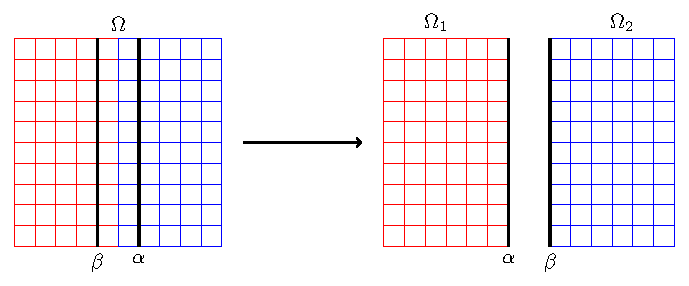
\includegraphics[width=\textwidth]{AOSM/TIKZ_AOSM_20230614.pdf}
%\end{figure}
%\end{frame}

\begin{frame}{Algebraic decomposition}

The subproblem on $\Omega_1$ is
\begin{equation*}
		\begin{bmatrix} A_{11} & A_{1 \Gamma} \\ A_{\Gamma 1} & A_{\Gamma \Gamma} + T_{2 \to 1} \end{bmatrix}
                            \begin{bmatrix} \vec{u}_1^{n+1} \\ \vec{u}_{1 \Gamma}^{n+1} \end{bmatrix}
                            = \begin{bmatrix} \vec{f}_1 \\ \vec{f}_\Gamma \end{bmatrix}
                            + \begin{bmatrix} ~ \\ -A_{\Gamma 2} \vec{u}_2^n + T_{2 \to 1} \vec{u}_{2 \Gamma}^n \end{bmatrix}
\end{equation*}
and the subproblem on $\Omega_2$ is
\begin{equation*}
       \begin{bmatrix} A_{22} & A_{2 \Gamma} \\ A_{\Gamma 2} & A_{\Gamma \Gamma} + T_{1 \to 2} \end{bmatrix}
                            \begin{bmatrix} \vec{u}_2^{n+1} \\ \vec{u}_{2 \Gamma}^{n+1} \end{bmatrix}
                            = \begin{bmatrix} \vec{f}_2 \\ \vec{f}_\Gamma \end{bmatrix}
                            + \begin{bmatrix} ~ \\ -A_{\Gamma 1} \vec{u}_1^n + T_{1 \to 2} \vec{u}_{1 \Gamma}^n \end{bmatrix}.
\end{equation*}

$\vec{u}_\Gamma$ appears in both subproblems since the interface is shared between the two subdomains.
These copies are distinct and must be recombined in some way at the end, for example:
\begin{equation*}
	\vec{u}_\Gamma = \frac{\vec{u}_{1 \Gamma} + \vec{u}_{2 \Gamma} }{2}.
\end{equation*}
\end{frame}

\begin{frame}{Transmission conditions}

Transmission conditions are boundary conditions of the subdomains.
Algebraically, they are implemented through the matrices $T_{1 \to 2}$ (which dictates how information passes \textit{from} $\Omega_1$ \textit{to} $\Omega_2$) and $T_{2 \to 1}$ ($\Omega_2$ to $\Omega_1$).

So far, we've seen Dirichlet boundary conditions on the subdomains, which is equivalent to $T=0$.

\end{frame}

% OSM? incl. algebraic transmission conditions
\begin{frame}{Options for transmission conditions}

\begin{itemize}
\item Dirichlet boundary conditions, equivalent to $T=0$
\item Neumann boundary conditions, allow minimal overlap
\item Optimized Robin boundary conditions:
\begin{equation*}
	\frac{\partial \vec{u}_1^{n+1}}{\partial x} - p \vec{u}_1^{n+1} = \frac{\partial \vec{u}_2^{n}}{\partial x} - p \vec{u}_2^{n}
\end{equation*}
for some $p$ optimized using Fourier analysis
\item Absorbing boundary conditions, equivalent to using Schur complements:
\begin{equation*}
	T_{i \to j} = S_{i \to j} := -A_{\Gamma i} A_{ii}^{-1} A_{i \Gamma}
\end{equation*}
\end{itemize}
With absorbing boundary conditions, the method becomes direct.
However, the Schur complements are expensive to compute and in general dense.

\end{frame}

\begin{frame}{Overview}

Schwarz methods play an important role in parallel computing.

The current research directions for domain decomposition methods include issues with 
\begin{itemize}
\item crosspoints (where three or more subdomains meet);
\item scalability (adding more processors should improve efficiency), and;
\item convergence rates (effectiveness of each iteration).
\end{itemize}

The work presented here aims to tackle this last point by finding new types of transmission conditions.
\end{frame}

\section{Adaptive optimized Schwarz methods} % 20 min

% predictor-corrector formulation
\begin{frame}{Schwarz method with adaptive transmission conditions}

Let $T_{i \to j}$ change at each iteration, so that the transmission conditions adapt.
We can formulate such a Schwarz method, acting only on $\vec{d}_i^{n+1} = \vec{u}_i^{n+1} - \vec{u}_i^n$, as
\begin{align*}
	\begin{bmatrix} A_{ii} & A_{i \Gamma} \\ A_{\Gamma i} & A_{\Gamma \Gamma} + T_{j \to i}^{n+1} \end{bmatrix}
	\begin{bmatrix} \vec{d}_i^{n+1} \\ \vec{d}_{i \Gamma}^{n+1} \end{bmatrix}
	= & \begin{bmatrix} ~ \\ -A_{\Gamma j} \vec{d}_j^n + T_{j \to i}^{n+1} \vec{d}_{j \Gamma}^n \end{bmatrix} \\
	& - \begin{bmatrix} ~ \\ \Delta T_{j \to i}^n \left ( \vec{u}_{i \Gamma}^n - \vec{u}_{j \Gamma}^{n-1} \right ) \end{bmatrix},
\end{align*}
where $i=1,2$, $j=3-i$, and $\Delta T_{j \to i}^n$ represents the update to the transmission condition $T_{j \to i}^n$ at this step,
\begin{equation*}
	T_{j \to i}^{n+1} = T_{j \to i}^n + \Delta T_{j \to i}^n.
\end{equation*}
\end{frame}

\begin{frame}{Condensing the iteration}

We can condense these iterations to express them as only acting on the difference at the interface.
First we note from the first row of blocks that
\begin{equation*}
	\vec{d}_i^{n+1} = -A_{ii}^{-1} A_{i \Gamma} \vec{d}_{i \Gamma}^{n+1},
\end{equation*}
and so likewise
\begin{equation*}
	\vec{d}_j^{n} = -A_{jj}^{-1} A_{j \Gamma} \vec{d}_{j \Gamma}^{n}.
\end{equation*}
Combining with the second row of blocks gives
\begin{align*}
	\left ( A_{\Gamma \Gamma} + S_{i \to j} + T_{j \to i}^{n+1} \right ) \vec{d}_{i \Gamma}^{n+1} =
	& \left ( T_{j \to i}^{n+1} - S_{j \to i} \right ) \vec{d}_{j \Gamma}^n \\
	& - \Delta T_{j \to i}^n \left ( \vec{u}_{i \Gamma} - \vec{u}_{j \Gamma}^{n-1} \right ).
\end{align*}
(Recall $S_{i \to j} = -A_{\Gamma i} A_{ii}^{-1} A_{i \Gamma}$)
\end{frame}

\begin{frame}{Difference between $T$ and $S$}
Notice the difference between the $T$ and $S$ matrices in these systems.
If we represent this difference as
\begin{equation*}
	E_{i \to j}^{n+1} := T_{i \to j}^{n+1} - S_{i \to j},
\end{equation*}
and write $\hat{A} := A_{\Gamma \Gamma} + S_{1 \to 2} + S_{2 \to 1}$, the Schur complement of the full system, then these systems become
\begin{equation*}
	\left ( \hat{A} + E_{i \to j}^{n+1} \right ) \vec{d}_{j \Gamma}^{n+1} = E_{i \to j}^{n+1} \vec{d}_{i \Gamma}^n - \Delta T_{i \to j}^n \left ( \vec{u}_{j \Gamma}^n - \vec{u}_{i \Gamma}^{n-1} \right ).
\end{equation*}
The matrix $E_{i \to j}^{n+1}$ is as expensive to calculate as the Schur complement, meaning this system is not practical.
However, it has immense theoretical value.
\end{frame}

\begin{frame}{Action of $E$}
\begin{equation*}
	E_{i \to j}^{n+1} \vec{d}_{i \Gamma}^n = -A_{\Gamma i} \vec{d}_i^n + T_{i \to j}^{n+1} \vec{d}_{i \Gamma}^n
\end{equation*}
\textit{A standard Schwarz method will compute vector pairs} $\left ( \vec{d}, E \vec{d} \right )$.
The vectors $\vec{d}$ are needed to find the solutions, while the vectors $E \vec{d}$ are found in the right hand sides of the systems to be solved.
We can use these vector pairs to approximate $E$ without calculating it.

Each vector pair gives a rank one approximation of $E$:
\begin{equation*}
	E \approx \frac{E \vec{d} \vec{d}^\top}{\norm{\vec{d}}_2^2} = E \frac{\vec{d}}{\norm{\vec{d}}} \frac{\vec{d}^\top}{\norm{\vec{d}}} = E \vec{w} \vec{w}^\top.
\end{equation*}
To combine these rank one matrices, we apply \textbf{modified Gram-Schmidt} to the vectors $\vec{d}$ and a commenserate process to the vectors $E \vec{d}$.
\end{frame}

% IAA algo + lemma
\begin{frame}
\begin{algorithm}[H]
	\caption{Iterative action approximation ($\iaa$) \\ $[V_n,W_n]=\iaa \left ( \set{\vec{d}_k}_{k=1}^n, E \right )$}
	\begin{algorithmic}[1]
		\State Inputs: $\set{\vec{d}_k}_{k=1}^{n} \subset \bbr^M$, $E \in \bbr^{M \times M}$
		\State $\alpha_1 := 1 / \norm{\vec{d}_1}$, $\vec{w}_1 := \alpha_1 \vec{d}_1$, $\vec{v}_1 := \alpha_1 E \vec{d}_1$
		\For{$k=2 : n$}
			\State $\vec{w}_k := \vec{d}_k$, $\vec{v}_k := E \vec{d}_k$
			\For{$i=1 : k-1$}
				\State $h \gets \langle \vec{w}_i, \vec{w}_k \rangle$, $\vec{w}_k \gets \vec{w}_k - h \vec{w}_i$
				\State $\vec{v}_k \gets \vec{v}_k - h \vec{v}_i$ \label{line: implicit}
			\EndFor
			\State $\alpha_k := 1 / \norm{\vec{w}_k}$, $\vec{w}_k \gets \alpha_k \vec{w}_k$, $\vec{v}_k \gets \alpha_k \vec{v}_k$
		\EndFor
		\State $W_{n} = \begin{bmatrix} \vec{w}_1 & \vec{w}_2 & \dots & \vec{w}_{n} \end{bmatrix}$, $V_{n} = \begin{bmatrix} \vec{v}_1 & \vec{v}_2 & \dots & \vec{v}_{n} \end{bmatrix}$
		\State $V_{n} W_{n}^\top \approx E$
	\end{algorithmic}
	\label{alg: IAA}
\end{algorithm}
\end{frame}

\begin{frame}{Properties of the IAA}
\begin{lemma} \label{lem: iaa}
%	Let $\mathcal{S}=\set{\vec{x}_k}_{k=1}^n \subset \bbr^M$ be a set of linearly independent vectors, $E \in \bbr^{M \times M}$ a matrix.
%	Let $[V_n,W_n]=\iaa(\mathcal{S},E)$ with columns $\vec{v}_k$ and $\vec{w}_k$, respectively.
	Let $E^1 := E$ and let $E^{k+1} := E^k - \vec{v}_k \vec{w}_k^\top$.
	Then
	\begin{align*}
		E^{k+1} = & E (I - W_k W_k^\top), \\
		\vec{v}_k = & E \vec{w}_k = E^k \vec{w}_k
	\end{align*}
	for $1 \leq k \leq n$, where $W_k$ is the first $k$ columns of $W_n$.
\end{lemma}

That is, the updates to $E$ increase its nullspace and preserve the relation between $\vec{w}$ and $\vec{v}$, which is the relation between $\vec{d}$ and $E \vec{d}$.
\end{frame}

\begin{frame}{Other fun facts about the $\iaa$}

\begin{itemize}
\item The vectors $\vec{w}_k$ form an orthonormal basis of a Krylov subspace % nb: include defn of this subspace?
\item Each subdomain has its own set of $\vec{w}_k$ and its own Krylov subspace
\item The vectors $\vec{v}_k$ are \textit{not} orthogonal
\end{itemize}
\end{frame}

% choice of adaptive transmission conditions + altAOSM + solve ladder(s?)
\begin{frame}{Choice of adaptive transmission conditions}

This gives us a rank one update to the transmission conditions:
\begin{equation*}
	\Delta T_{i \to j}^n = - \vec{v}_i^k \left ( \vec{w}_i^k \right )^\top.
\end{equation*}

This choice of $\Delta T$ eliminates the product $E_{i \to j}^{n+1} \vec{d}_{i \Gamma}^n$ from the earlier systems.
We must now solve
\begin{equation*}
	\begin{bmatrix} A_{jj} & A_{j \Gamma} \\ A_{\Gamma j} & A_{\Gamma \Gamma} + T_{i \to j}^{n+1} \end{bmatrix}
	\begin{bmatrix} \vec{d}_j^{n+1} \\ \vec{d}_{j \Gamma}^{n+1} \end{bmatrix}
	= (\vec{w}_i^n)^\top \left ( \vec{u}_{j \Gamma}^n - \vec{u}_{i \Gamma}^{n-1} \right )\begin{bmatrix} ~ \\ \vec{v}_i^n \end{bmatrix}
\end{equation*}
at every step.
\end{frame}

\begin{frame}
\begin{algorithm}[H]
	\caption{altAOSM: AOSM applied to multiplicative Schwarz} %nb: include function defn like iaa?
	\label{alg: alt}
	\begin{algorithmic}[1]
		\State Start with initial transmission conditions $T_{1 \to 2}^1$ and $T_{2 \to 1}^1$
		\State Make initial guess $\vec{u}_{1 \Gamma}^0$
		\State Calculate $\vec{u}_1^0 = A_{11}^{-1} ( \vec{f}_1 - A_{1 \Gamma} \vec{u}_{1 \Gamma}^0 )$
		\State Solve for $\vec{u}_2^1$ and $\vec{u}_{2 \Gamma}^1$, then for $\vec{u}_1^2$ and $\vec{u}_{1 \Gamma}^2$
		\State Calculate $\vec{d}_{1 \Gamma}^2 = \vec{u}_{1 \Gamma}^2 - \vec{u}_{1 \Gamma}^0$ and $\vec{d}_1^2$ and set $n=2$
		\While{$\norm{ \vec{d}_{1 \Gamma}^n } + \norm{ \vec{d}_{2 \Gamma}^{n-1} } \geq tol$}
			\For{$i=1 : 2$ (and $j=3-i$)}
				\State Run an iteration of $\iaa$
				\State Set $\Delta T_{i \to j}^n = - \vec{v}_i^n (\vec{w}_i^n)^\top$
				\State Solve for $\vec{d}_{j \Gamma}^{n+1}$ and $\vec{d}_j^{n+1}$
				\State $\vec{u}_j^{n+1} := \vec{u}_j^{n-1} + \vec{d}_j^{n+1}$, $\vec{u}_{j \Gamma}^{n+1} := \vec{u}_{j \Gamma}^{n-1} + \vec{d}_{j \Gamma}^{n+1}$
				\State $n \gets n+1$
			\EndFor
		\EndWhile
		\State Output: $\vec{u} = [ \vec{u}_1^n \ ; \ (\vec{u}_{1 \Gamma}^n + \vec{u}_{2 \Gamma}^{n-1})/2 \ ; \ \vec{u}_2^{n-1} ]$
	\end{algorithmic}
\end{algorithm}
\end{frame}

\begin{frame}
\centering
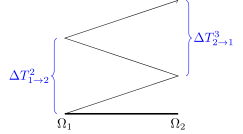
\includegraphics[width=0.45\textwidth]{AOSM/TIKZ_AOSM_20230614_3.png}
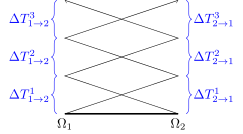
\includegraphics[width=0.45\textwidth]{AOSM/TIKZ_AOSM_20230614_4.png}
\end{frame}

% Galerkin condition for AOSM
\begin{frame}{AOSM Galerkin condition}

\begin{theorem} \label{thm: opt}
If $\hat{A} + E_{i \to j}^{n+1}$ is invertible, then the update to the solution due to an AOSM is $$\vec{d}_{j \Gamma}^{n+1} = \AijE \vec{x},$$ where
$\vec{x} \in  \Span(W_i^n)$ such that the residual of
\begin{align*}
	& \left ( I - \left ( \hat{A} + E_{i \to j}^{n+1} \right )^{-1} E_{i \to j}^{n+1} \right ) \vec{u}_\Gamma \\
	& = \left ( \hat{A} + E_{i \to j}^{n+1} \right )^{-1} \left ( \vec{f}_\Gamma - A_{\Gamma j} A_{jj}^{-1} \vec{f}_j - A_{\Gamma i} A_{ii}^{-1} \vec{f}_i \right )
\end{align*}
applied to $\vec{u}_{i \Gamma}^{n-1} + \vec{x}$ is orthogonal to $\Span(W_i^n)$. 
\end{theorem}
\end{frame}

\begin{frame}{AOSM Galerkin condition}

\begin{enumerate}
\item The solution on the interface, $\vec{u}_\Gamma$, solves a system $B \vec{u}_\Gamma = \vec{b}$
\item There is a vector $\vec{x} \in \Span(W_i^n)$ such that $B(\vec{u}_{i \Gamma}^{n-1} + \vec{x}) - \vec{b}$ is orthogonal to $\Span(W_i^n)$
\item The vector $\vec{d}_{j \Gamma}^{n+1}$, determined by the AOSM, is equal to $$\vec{d}_{j \Gamma}^{n+1} = \AijE \vec{x}$$
\end{enumerate}
\end{frame}

% numerical results: basic comparison with GMRES
\section{Numerical results of AOSM}

\begin{frame}{Simple comparison with other methods}

\begin{equation*}
	\begin{cases} \Delta u(x,y) = f(x,y), & (x,y) \in \Omega = [-1,1] \times [-1,1], \\
		u(x,y) = g(x,y), & (x,y) \in \partial \Omega. % = \set{x=-1} \cup \set{x=1} \cup \set{y=-1} \cup \set{y=1} .
	\end{cases}
\end{equation*}

\begin{figure}
	\begin{columns}
	\column{0.6\linewidth}
	\begin{tikzpicture}
			\draw[step=1em,red] (0,0) grid (5em,10em);
			\draw[step=1em,blue] (5em,0) grid (10em,10em);
			\node[below] at (5em,0) {$x_\Gamma$};
			\draw[very thick, black] (5em,0) -- (5em,10em);
			\node[above] at (5em,10em) {$\Omega$};
			\draw[decorate,decoration={brace, amplitude=1em, raise=0.5em}] (0,0) -- (0,10em) node[midway, xshift=-2.5em] {100};
			\draw[decorate, decoration={brace, amplitude=0.5em, mirror, raise=0.5em}] (0,0) -- (4em,0) node[midway, yshift=-2em] {49};
			\draw[decorate, decoration={brace, amplitude=0.5em, mirror, raise=0.5em}] (6em,0) -- (10em,0) node[midway, yshift=-2em] {50};
	\end{tikzpicture}
	\column{0.3\linewidth}
	\caption{$100 \times 100$ evenly spaced grid split into two subdomains along the 50th value of $x$}
	\end{columns}
\end{figure}
\end{frame}

\begin{frame}{Simple comparison with other methods}
\begin{figure}
	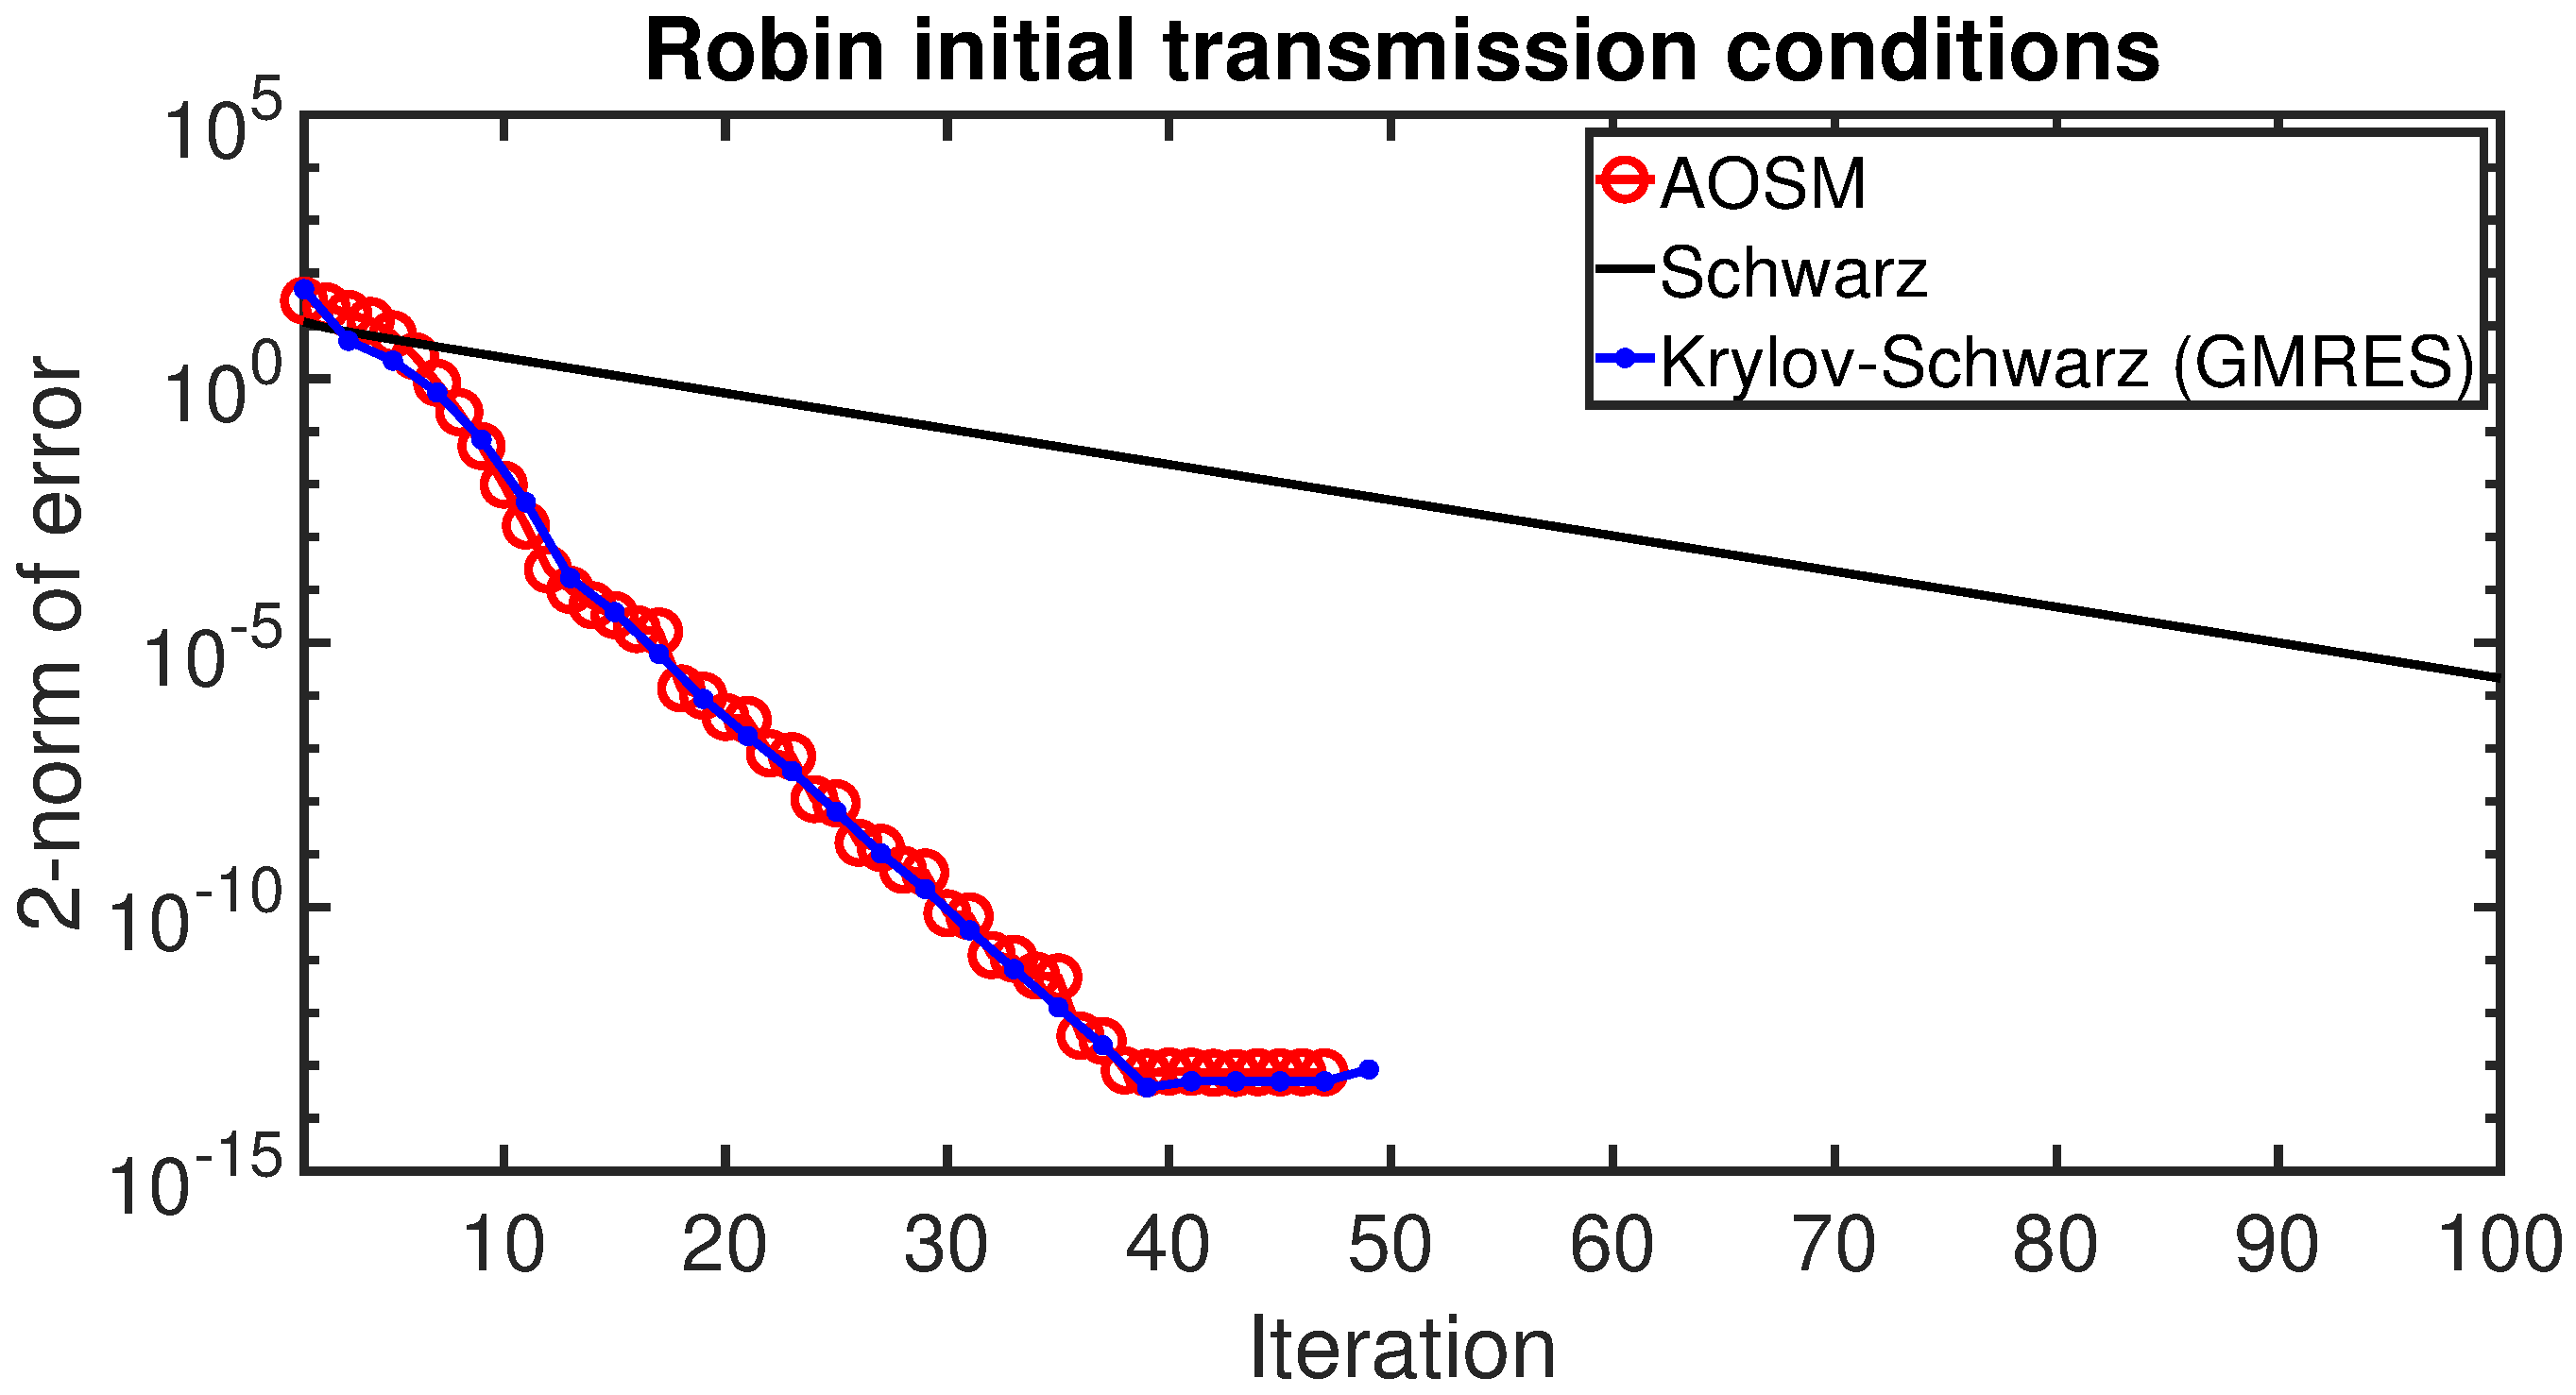
\includegraphics[width=\textwidth]{AOSM/PLOT_faltAOSMConv_Seminar1.eps}
	\caption{Comparison between Schwarz, AOSM and Krylov-Schwarz on simple elliptic PDE}
\end{figure}
\end{frame}

% multiple subdomains (Schur complements for red-black)
\begin{frame}[fragile]
\frametitle{Precursor to multiple subdomains: red-black decompositions}
\begin{figure}
	\centering
	\begin{tikzpicture}
		\matrix[row sep=1em, column sep=1em]{%, ampersand replacement=\amp]{
			\draw[step=1em,red] (0,0) grid (3em,10em);
			\draw[step=1em,blue] (3em,0) grid (5em,10em);
			\draw[step=1em,red] (5em,0em) grid (7em,10em);
			\draw[step=1em,blue] (7em,0em) grid (10em,10em);
			\node[below] at (3em,0) {$x_\Gamma$};
			\draw[very thick, black] (3em,0) -- (3em,10em);
			\node[below] at (5em,0) {$x_\Gamma$};
			\draw[very thick, black] (5em,0) -- (5em,10em);
			\node[below] at (7em,0) {$x_\Gamma$};
			\draw[very thick, black] (7em,0) -- (7em,10em);
			\node[above] at (5em,10em) {$\Omega$};
			& \draw[thick,black,->] (0,5em) -- (0.5,5em); &
			\draw[step=1em,red] (0,0) grid (3em,10em);
			\draw[step=1em,red] (5em,0em) grid (7em,10em);
			\node[above] at (5em,10em) {$\Omega_1$}; &
			\draw[step=1em,blue] (3em,0) grid (5em,10em);
			\draw[step=1em,blue] (7em,0em) grid (10em,10em);
			\node[above] at (5em,10em) {$\Omega_2$};
		\\};
	\end{tikzpicture}
	\caption{Splitting the $100 \times 100$ grid into four strips, then pairing the strips into two algebraic subdomains}
\end{figure}
\end{frame}

\begin{frame}{Comparison: stripwise}
\begin{figure}
	\centering
	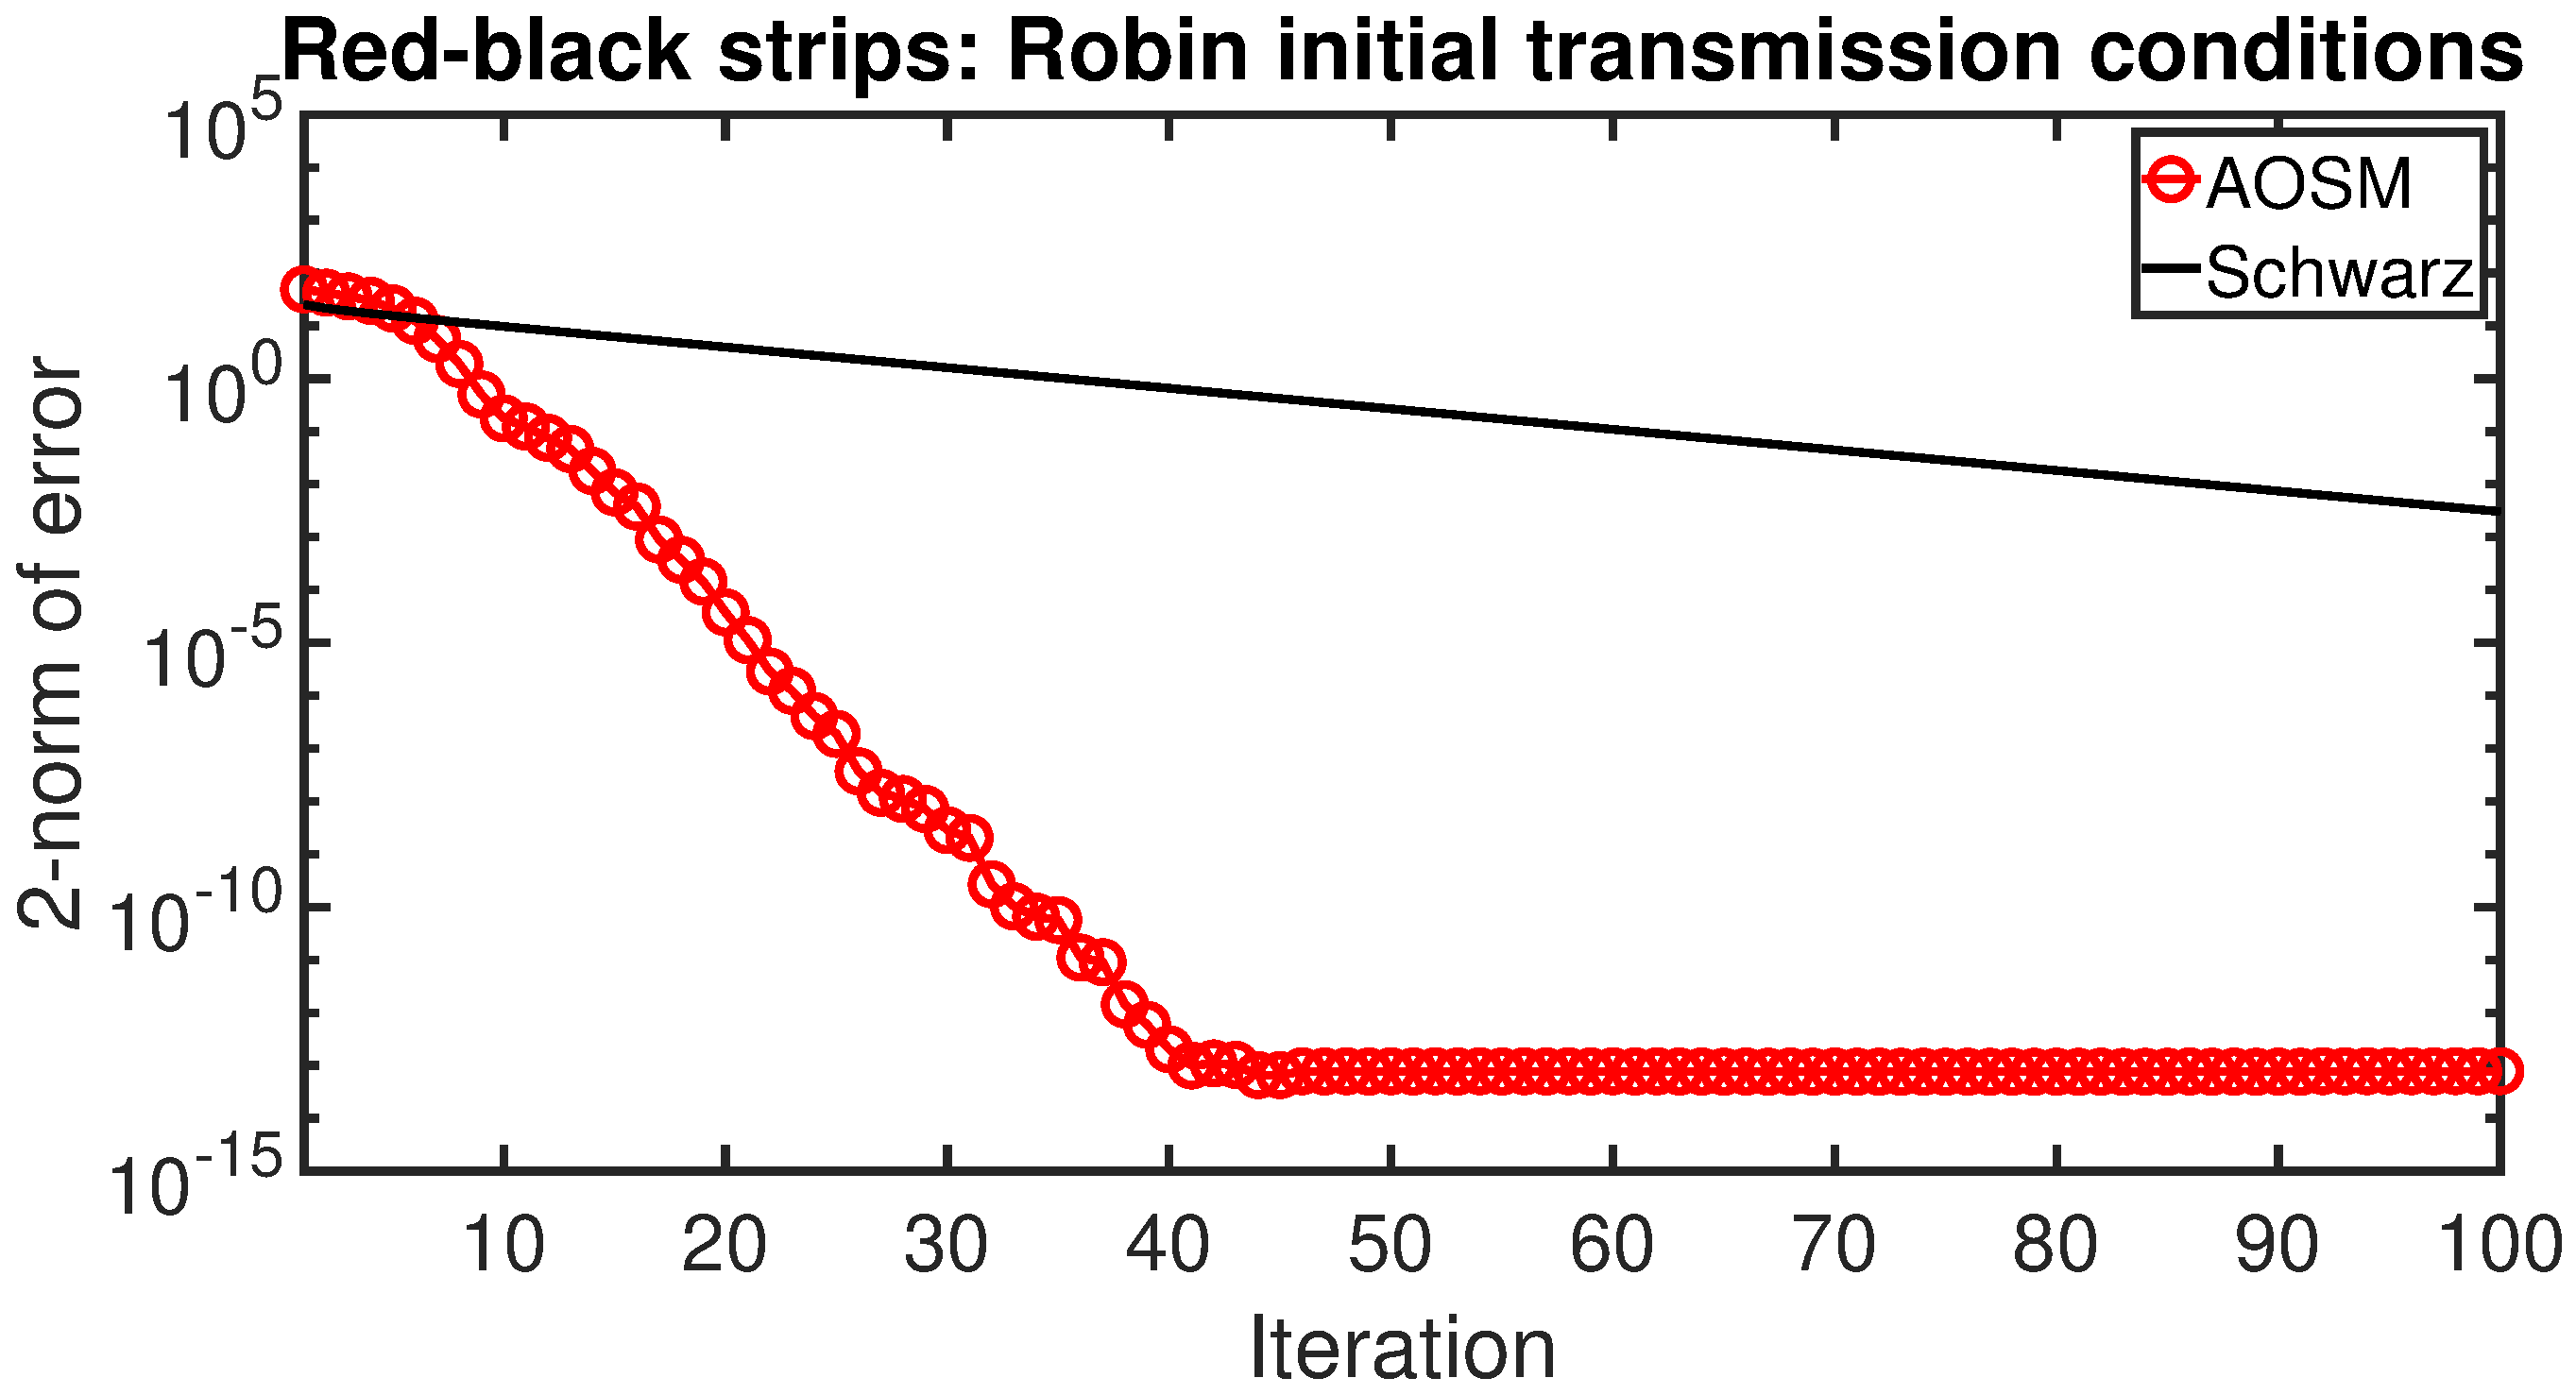
\includegraphics[width=\textwidth]{AOSM/PLOT_RedBlack_Seminar2.eps}
	\caption{Convergence for AOSM and Schwarz on the stripwise decomposition}
\end{figure}
\end{frame}

\begin{frame}{Adapted transmission conditions: stripwise}
\begin{figure}
	\centering
	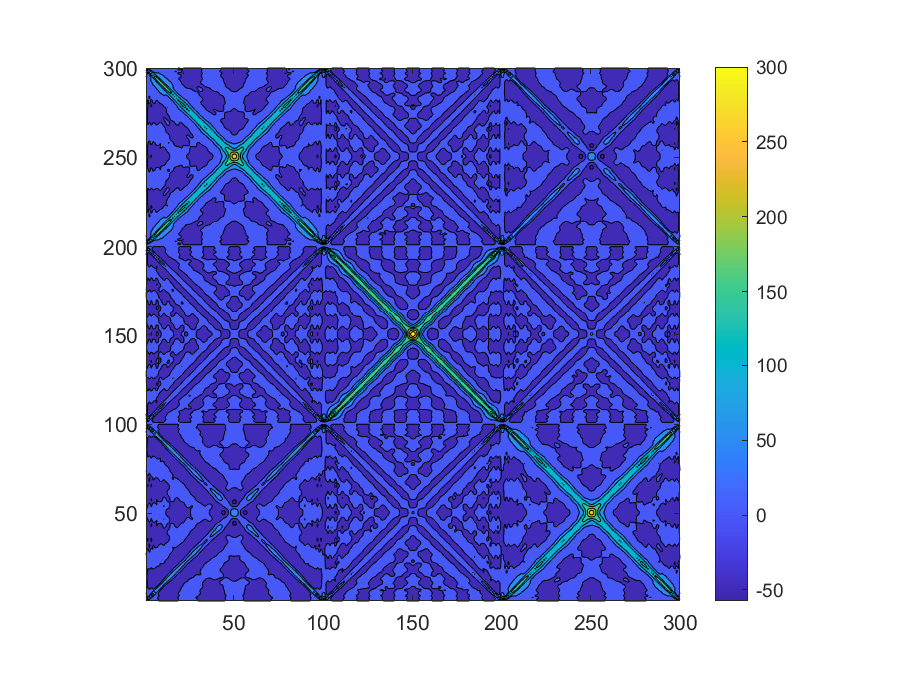
\includegraphics[width=0.8\textwidth]{AOSM/PLOT_RedBlack_T_Seminar3.eps}
	\caption{Matrix $T_{1 \to 2}$ from AOSM after convergence of stripwise example}
\end{figure}
\end{frame}

\begin{frame}{Heterogeneous elliptic PDE}
\begin{equation*}
	\begin{cases} -\nabla \left ( \alpha(x,y) \cdot \nabla u(x,y) \right ) = f(x,y), & (x,y) \in \Omega = [0,1] \times [0,1], \\
		u(x,y) = g(x,y), & (x,y) \in \partial \Omega. % = \set{x=-1} \cup \set{x=1} \cup \set{y=-1} \cup \set{y=1} .
	\end{cases}
\end{equation*}

\begin{figure}
	\begin{columns}
	\column{0.6\linewidth}
	\centering
	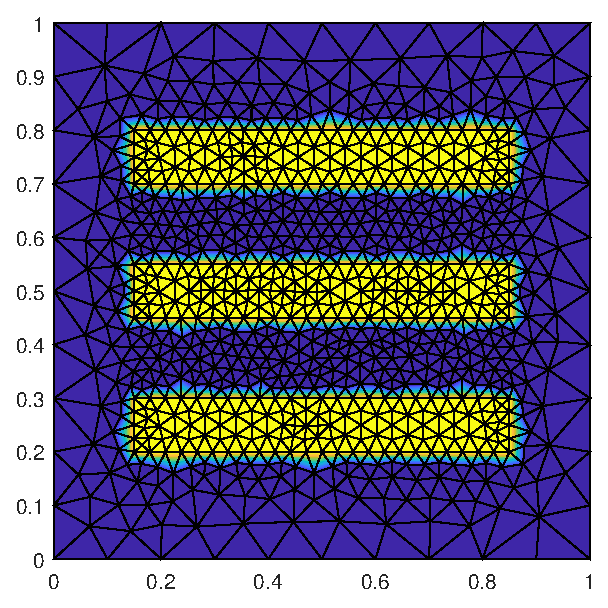
\includegraphics[height=0.6\textheight]{AOSM/PLOT_LonelandK_Seminar.eps}
	\column{0.3\linewidth}
	\caption{$\alpha(x,y)=1$ except along three thin channels where $\alpha(x,y)=1000$}
	\end{columns}
\end{figure}
\end{frame}

\begin{frame}{Unstructured grid}
\begin{figure}
	\begin{columns}
	\column{0.6\linewidth}
	\centering
	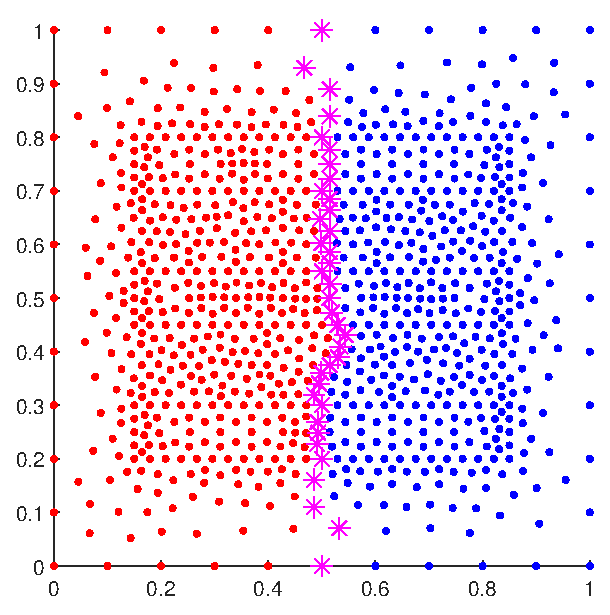
\includegraphics[height=0.6\textheight]{AOSM/PLOT_LonelandSubdomains_Seminar.eps}
	\column{0.3\linewidth}
	\caption{Splitting an unstructured grid into two subdomains}
	\end{columns}
\end{figure}
\end{frame}

\begin{frame}{First round of solves}
\begin{figure}
	\centering
	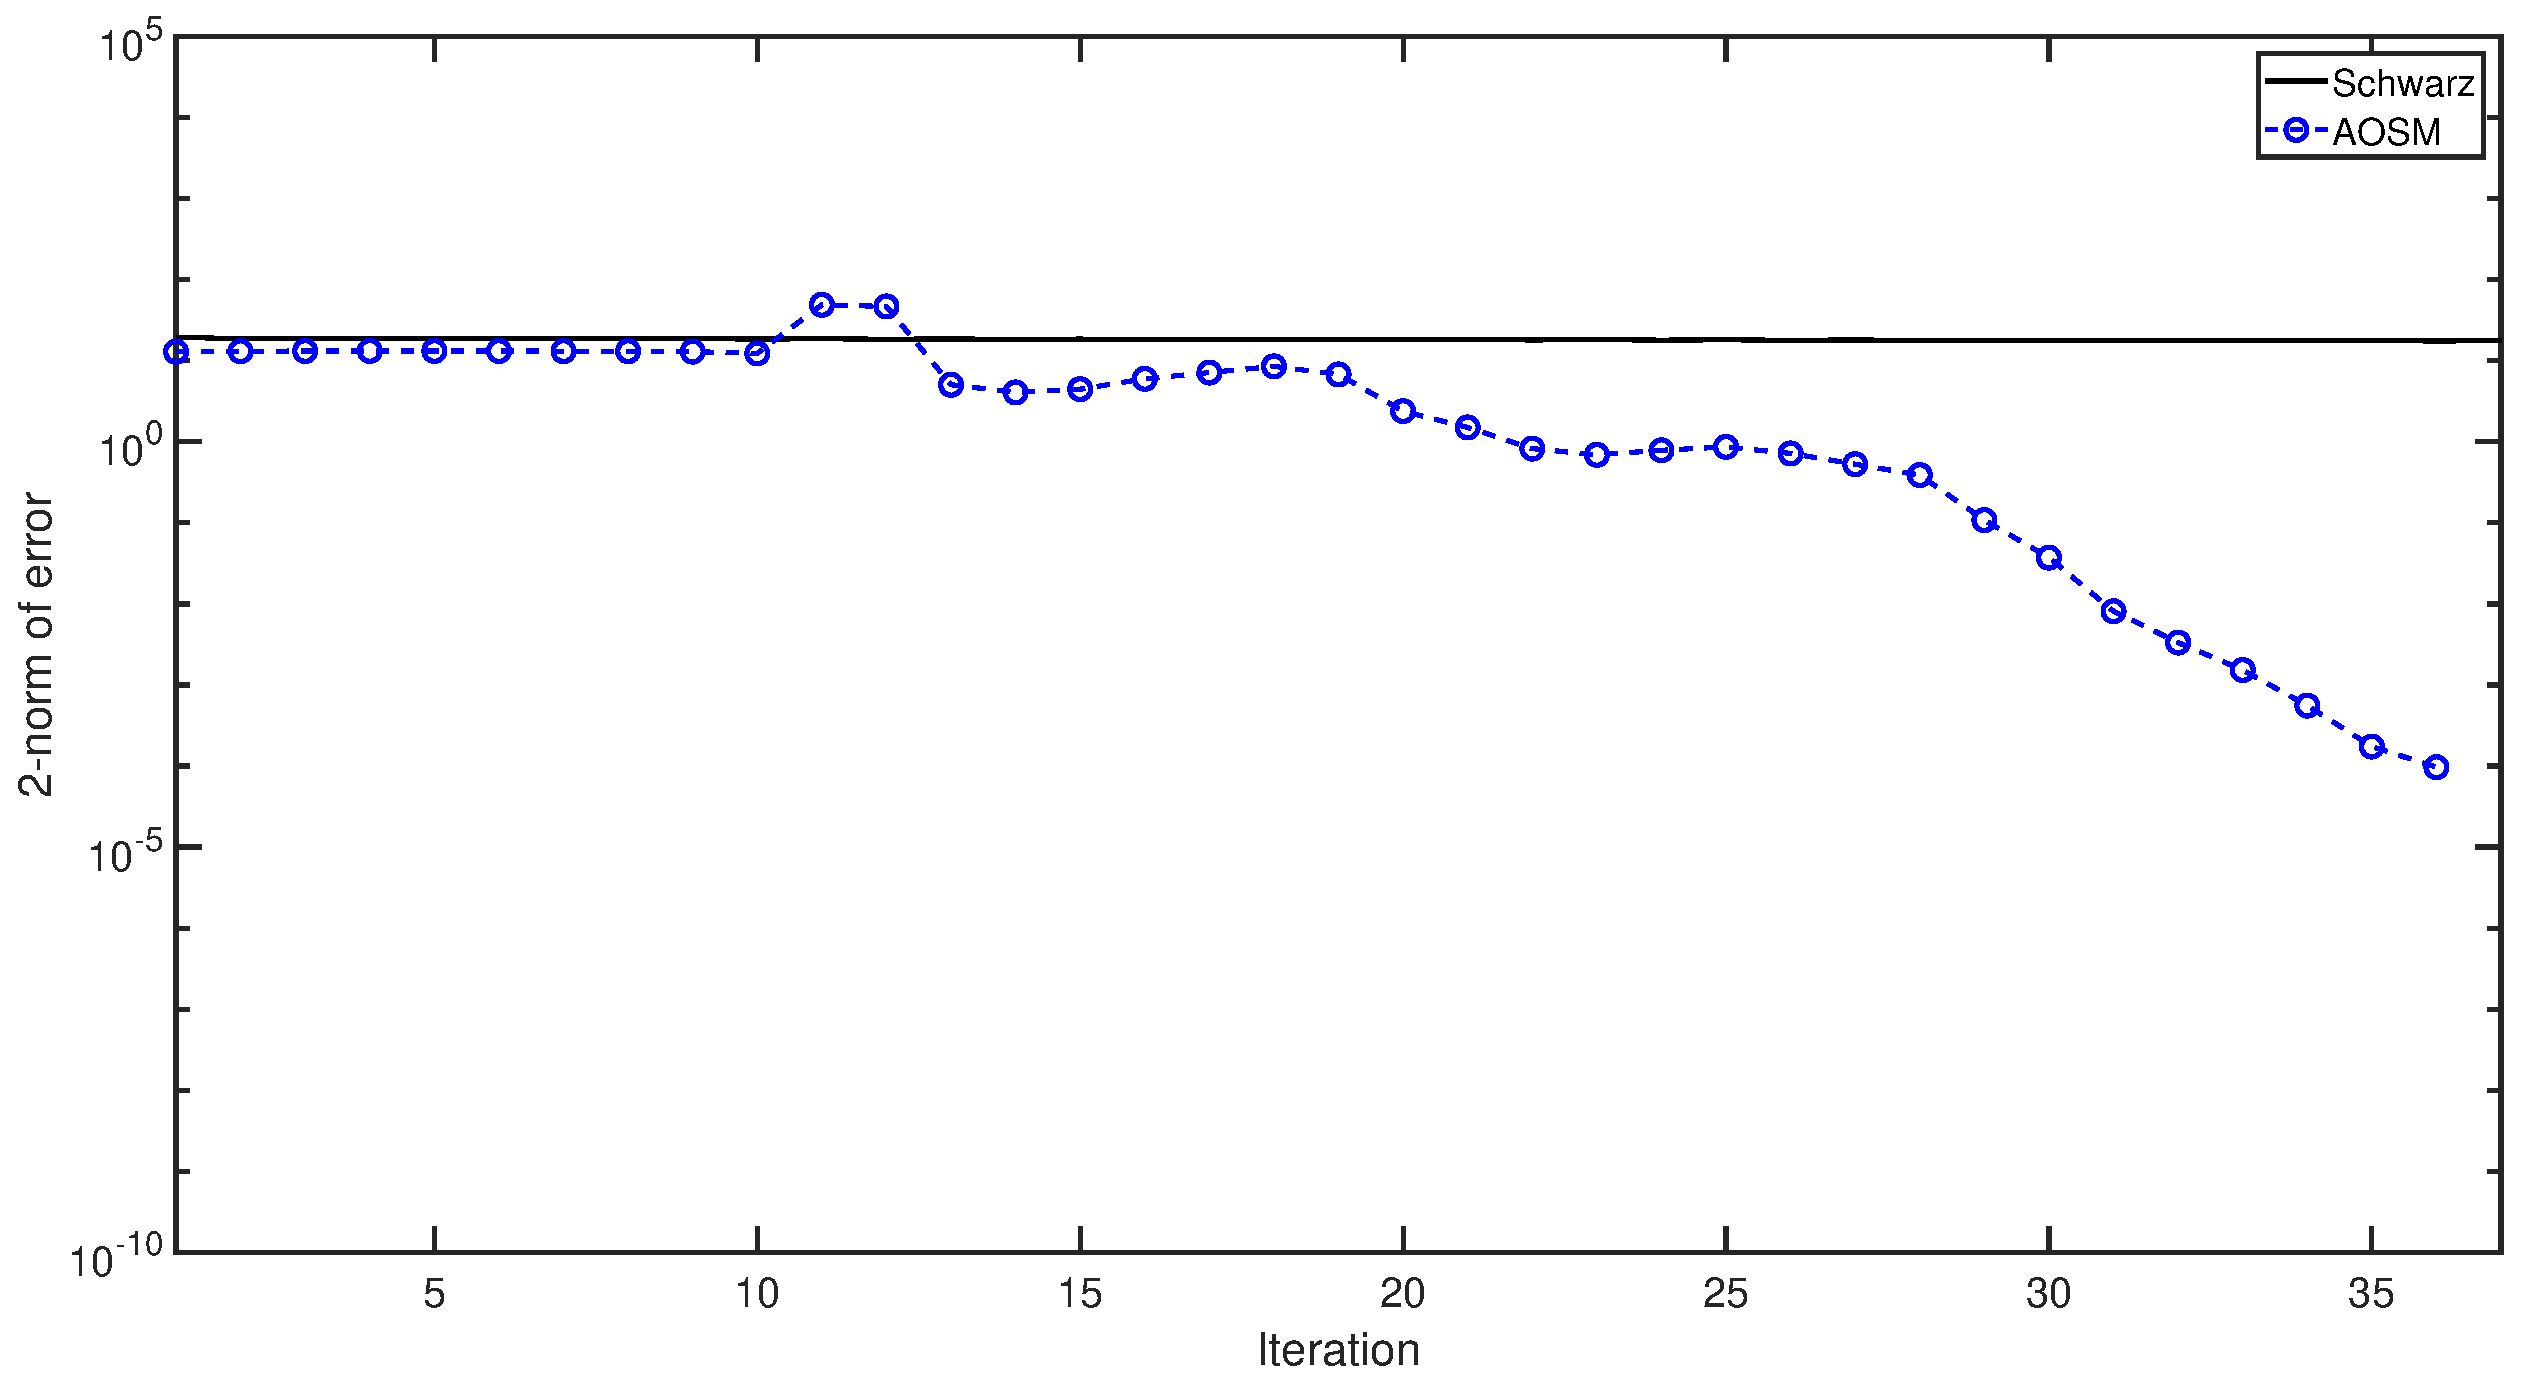
\includegraphics[width=\textwidth]{AOSM/PLOT_LonelandFirst_Seminar.eps}
	\caption{(Lack of) convergence for Schwarz and AOSM for heterogeneous elliptic PDE}
\end{figure}
\end{frame}

\begin{frame}{Second round of solves}
\begin{figure}
	\centering
	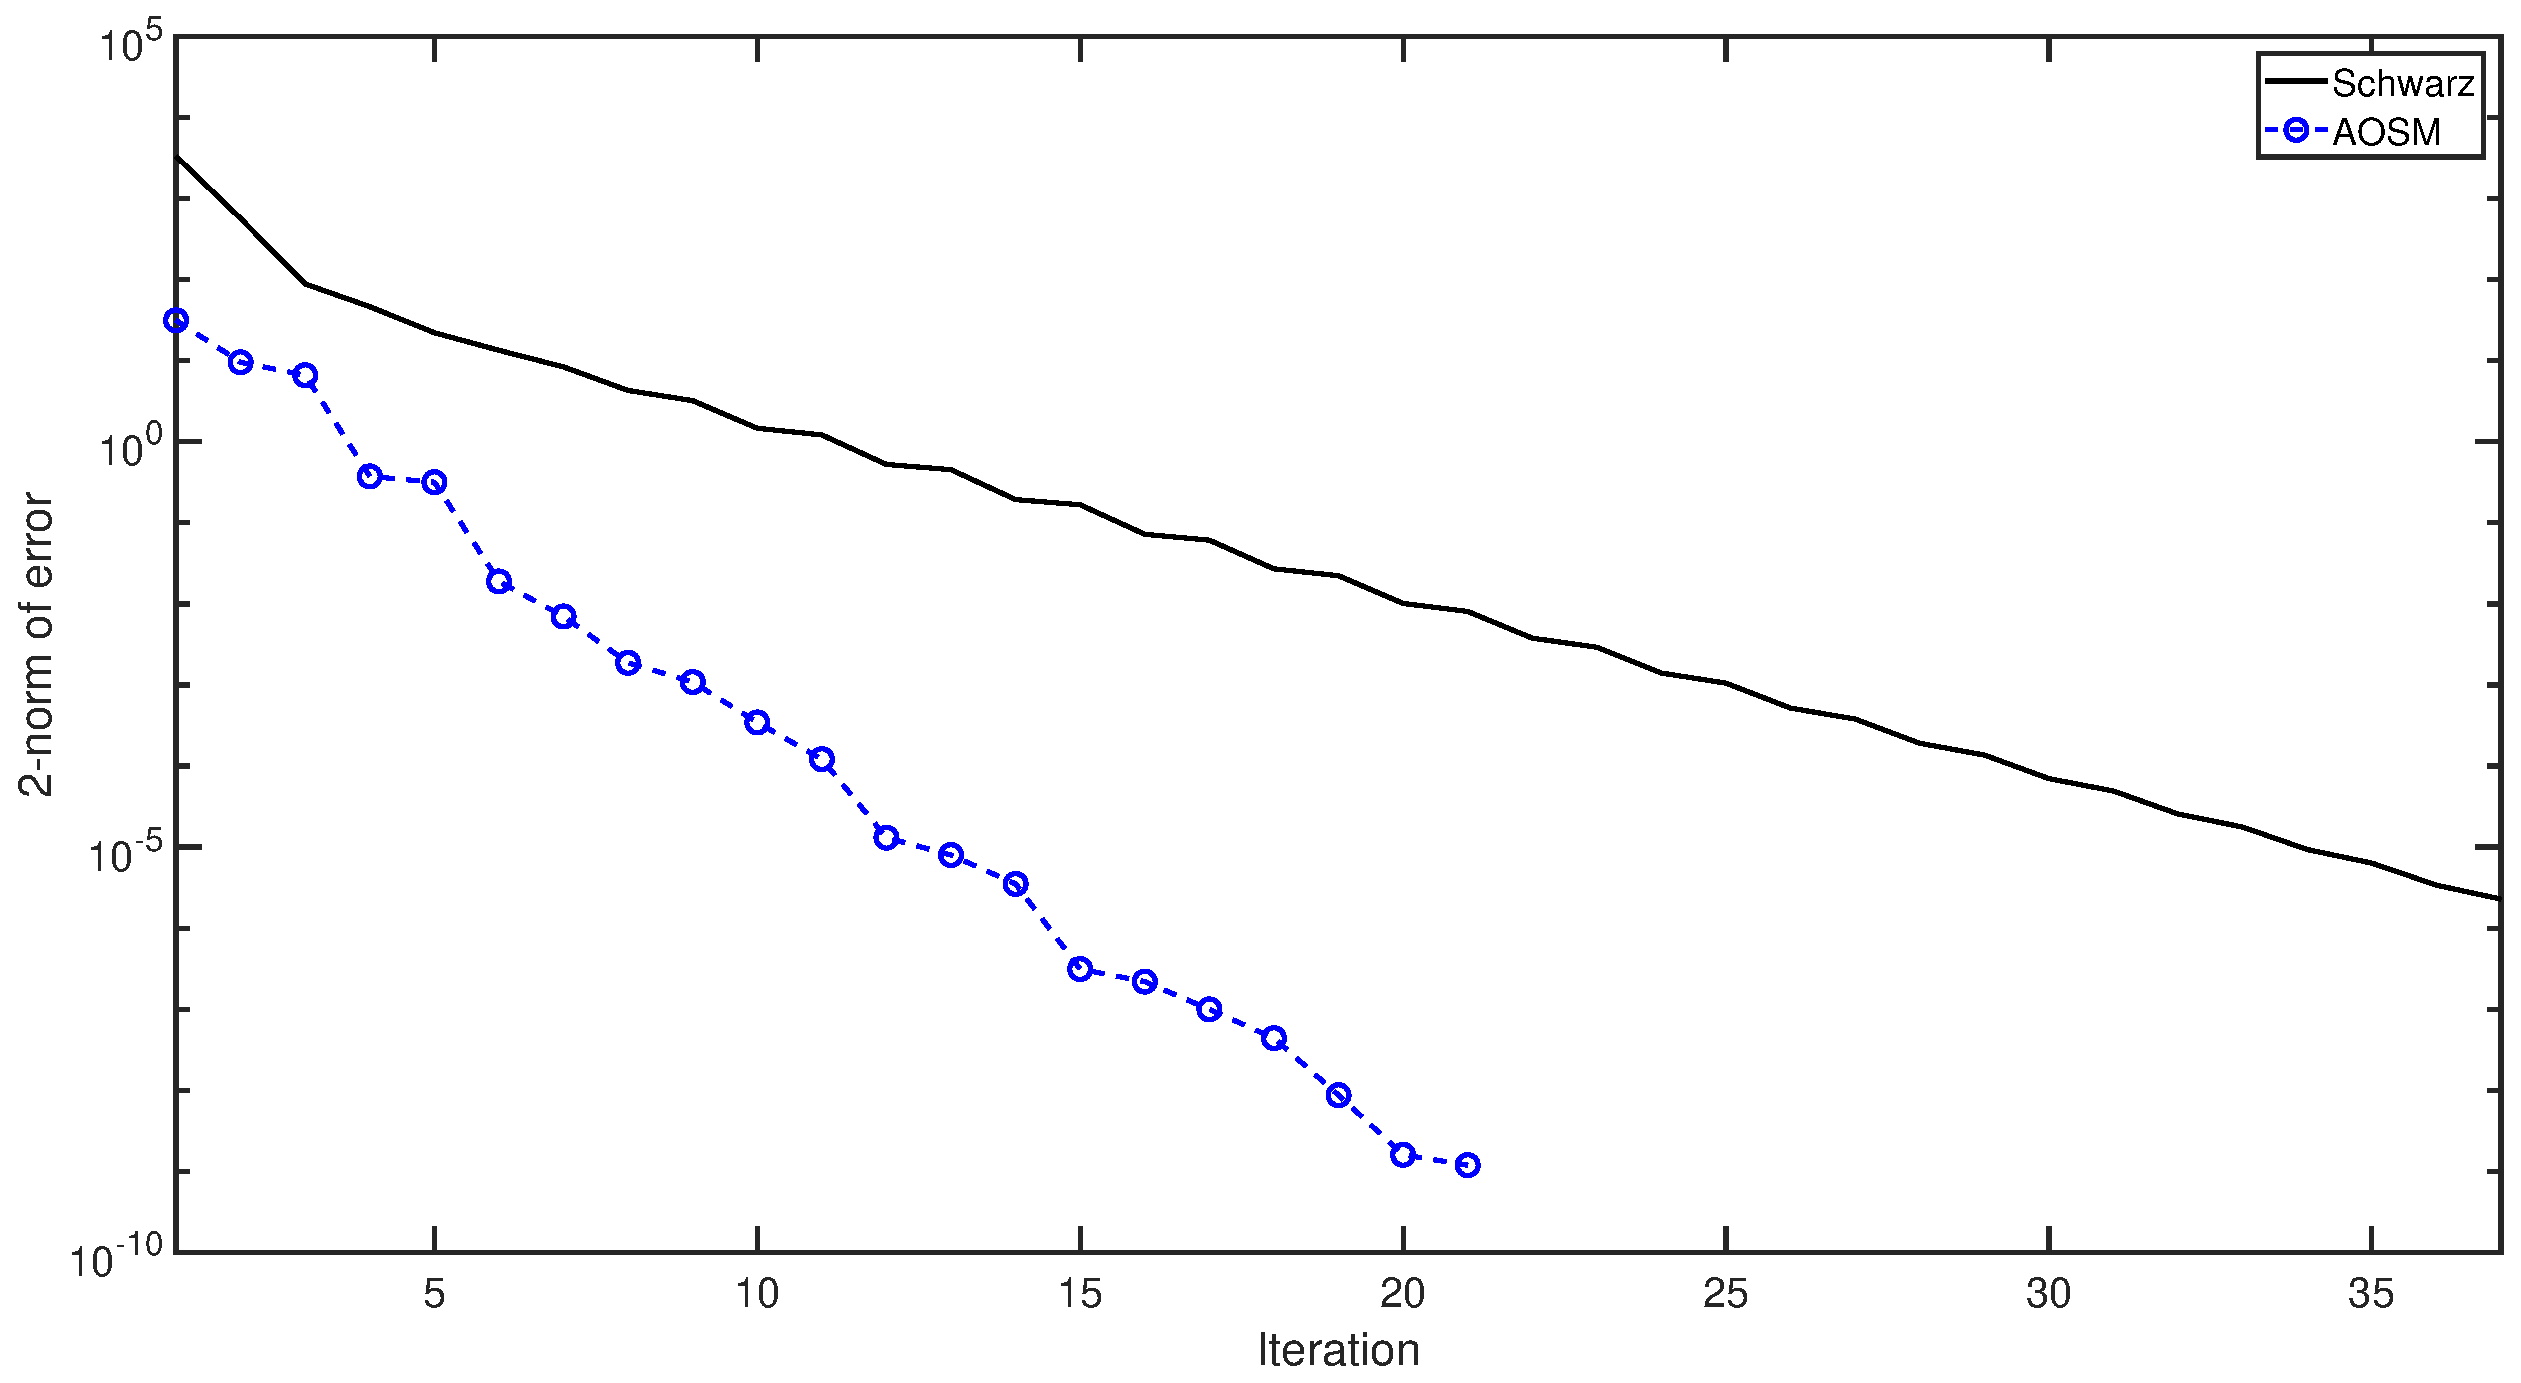
\includegraphics[width=\textwidth]{AOSM/PLOT_LonelandSecond_Seminar.eps}
	\caption{Convergence for Schwarz and AOSM using adapted transmission conditions}
\end{figure}
\end{frame}

\section{Future work}

\begin{frame}{AOSM difficulties: Crosspoints}

We need to generalize the AOSM for multiple subdomains.
We've already seen that we need new types of updates to the transmission conditions to account for the shape of the Schur complements.

A common problem with domain decomposition methods for multiple subdomains is \textbf{crosspoints}: points where three or more subdomains meet.
At this point, it is not clear how information should be transmitted.

Some new results have figured out workarounds for rectilinear grids (Chaudet-Dumas \& Gander, 2023).
More general techniques are needed.
\end{frame}

\begin{frame}{AOSM difficulties: Scalability}

Another common issue with domain decomposition methods is \textbf{scalability}.
A method in parallel computing is scalable if adding more processors always improves efficiency.

For domain decomposition methods, information from each subdomain must pass to every other subdomain, often multiple times.
This means that the computation time is limited by the length of the longest path through the network of subdomains.

Researchers have found multigrid methods can be combined with domain decomposition methods to overcome much of this issue.

\end{frame}

%\begin{frame}{New approximations of Schur complements}
%
%It's clear that the transmission conditions we're finding do not need to be so dense.
%For the multiple subdomains, it appears we can approximate the Schur complements with block diagonal matrices.
%
%We could also use completely different approximations to the rank one updates shown in these slides.
%For example, hierarchical decompositions.
%
%These changes require altering how the $T$ matrices are constructed, and will probably not have the same Galerkin condition as before.
%\end{frame}

% symmetrized cells
\begin{frame}[fragile]
\frametitle{Symmetrized cells}

As an alternative way to use AOSMs for multiple subdomains,
one can first prioritize optimizing the transmission conditions for each subproblem.

Isolate the subdomain and symmetrize it, i.e. make one or several \textit{virtual} copies of the subdomain.
Solve this subproblem repeatedly until the $T$ matrices have adapted.
Then redistribute the $T$ matrices to their appropriate subproblems.

\begin{figure}
	\centering
	\begin{tikzpicture}
		\matrix[row sep=1em, column sep=1em]{
			\draw[very thick,black] (0,0) -- (0,3) -- (3,3) -- (3,0) -- cycle;
			\filldraw[cyan] (0,0) -- (0,3) -- (3,3) -- (3,0) -- cycle;
			\foreach \x in {1,2} {
				\draw[black] (0,\x) -- (3,\x);
				\draw[black] (\x,0) -- (\x,3);}
			\pic at (1,1) {starred};
			\node[star, fill=magenta!30!black] at (1.5,1.5) {};
			&
			\draw[->, very thick, black] (0,1.5) -- (1.5,1.5);
			&
			\pic at (1,1) {starred};
			\node[star, fill=magenta!30!black] at (1.5,1.5) {};
			\foreach \x in {1,3} {
				\pic[xscale=-1] at (\x,1) {starred};
				\pic[yscale=-1] at (1,\x) {starred};
				\pic[xscale=-1, yscale=-1] at (\x,\x) {starred};}
			\pic[xscale=-1, yscale=-1] at (1,3) {starred};
			\pic[xscale=-1, yscale=-1] at (3,1) {starred};
			\foreach \x in {1,2} {
				\draw[black] (0,\x) -- (3,\x);
				\draw[black] (\x,0) -- (\x,3);}
		\\};
	\end{tikzpicture}
\end{figure}
\end{frame}

\begin{frame}{Conclusions}
\begin{itemize}
\item AOSMs give Krylov-Schwarz convergence rates without the extra computations.
\item Transmission conditions from AOSMs can be re-used to give fast convergence.
\item We need to generalize the AOSMs for different types of approximations of the Schur complement.
\item Symmetrized cells can be used to find the transmission conditions beforehand.
\end{itemize}
\end{frame}

\iffalse
% ASPIN/MSPIN/RASPEN
\begin{frame}{Schwarz as a fixed point iteration}

Schwarz methods can be represented as fixed point iterations:
\begin{equation*}
	u^{n+1} = g \left ( u^{n-1} \right ),
\end{equation*}
where $g(u)$ represents one iteration of a Schwarz method that takes boundary data from the input $u$.

The fixed point of $g$ is the solution on the first subdomain.
This is also the root of the function $f(u) = g(u) - u$.
We apply Newton's method:
\begin{equation*}
	u^* = u^{n-1} - J(u^{n-1})^{-1} f(u^{n-1}),
\end{equation*}
where $J$ is the Jacobian of the function $f$.
\end{frame}

\begin{frame}{Schwarz-Preconditioned Newton methods (Cai \& Keyes, 2001)}

This is equivalent to preconditioning Newton's method with a Schwarz method.

Let
\begin{equation*}
	f(u) = \begin{bmatrix} f_1(u_1, u_2) \\ f_2(u_1,u_2) \end{bmatrix}.
\end{equation*}
Then Newton's method tells us to solve the nonlinear problem
\begin{equation*}
	\begin{bmatrix} J_{11}^{(n+1)} & J_{12}^{(n+1)} \\ J_{21}^{(n+1)} & J_{22}^{(n+1)} \end{bmatrix} \begin{bmatrix} u_1^{n+1} - u_1^n \\ u_2^{n+1} - u_2^n \end{bmatrix} = \begin{bmatrix} f_1 \\ f_2 \end{bmatrix},
\end{equation*}
where $J_{ij}^{(n+1)}$ is the derivative of $f_i$ with respect to $u_j$ evaluated at $u_1^{n+1}$ and $u_2^{n+1}$.
\end{frame}

\begin{frame}{Schwarz-Preconditioned Newton methods (Cai \& Keyes, 2001)}

Preconditioning this with a parallel Schwarz method tells us to solve
\begin{equation*}
	\begin{bmatrix} J_{11}^{(n+1)} \\ & J_{22}^{(n+1)} \end{bmatrix} \begin{bmatrix} u_1^{n+1} - u_1^n \\ u_2^{n+1} - u_2^n \end{bmatrix} = \begin{bmatrix} f_1 \\ f_2 \end{bmatrix} - \begin{bmatrix} & J_{12}^{(n)} \\ J_{21}^{(n)} \end{bmatrix} \begin{bmatrix} u_1^{n} - u_1^{n-1} \\ u_2^{n} - u_2^{n-1} \end{bmatrix},
\end{equation*}
and completing the iteration by solving
\begin{equation*}
	\begin{bmatrix} J_{11}^{(n+1)} \\ & J_{22}^{(n+1)} \end{bmatrix}^{-1} \begin{bmatrix} J_{11}^{(n+1)} & J_{12}^{(n+1)} \\ J_{21}^{(n+1)} & J_{22}^{(n+1)} \end{bmatrix} \begin{bmatrix} u_1^* - u_1^n \\ u_2^* - u_2^n \end{bmatrix}
	= \begin{bmatrix} f_1(u_1^{n+1},u_2^{n+1}) \\ f_2(u_1^{n+1},u_2^{n+1}) \end{bmatrix}.
\end{equation*}

\end{frame}

\section{Alternate minimization in phase-field fracture models} % 15 min

\begin{frame}{Brittle fracture}

\begin{figure}
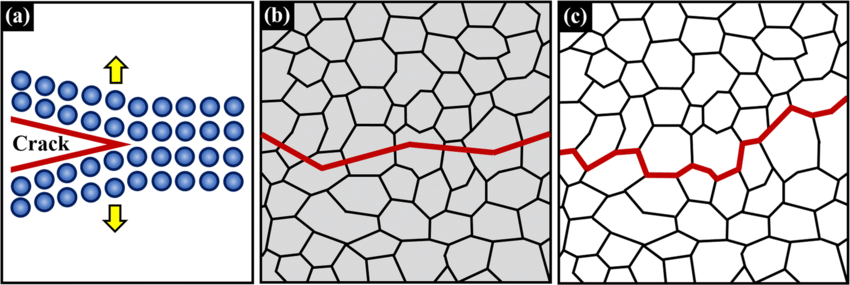
\includegraphics[width=\textwidth]{Fractures/FIG_BrittleFracture.png}
\caption{Crack propagation in brittle material, image taken from ResearchGate, uploaded by Dana Ashkenazi}
\end{figure}
\end{frame}

% phase-field fracture model
\begin{frame}{Phase-field fracture model}

\begin{equation*}
	E_\ell(u,\alpha) = \int \frac{1}{2} (1 - \alpha)^2 A e(u) \cdot e(u) dx + \frac{G_c}{4 c_w} \int \frac{w(\alpha)}{\ell} + \ell \abs{\nabla \alpha}^2 dx
\end{equation*}
\begin{itemize}
\item $u$ is a vector field which defines the displacement
\item $\alpha$ is a scalar field that is 0 away from the crack and 1 on the crack
\item $e(u)$ is the strain tensor, $A$ the stiffness tensor
\item $\ell$ determines the accuracy of the approximation of the Hausdorff measure of the crack
\item $w(0)=0$, $w(1)=1$, $w'(x) \geq 0$, $w \in C^1(0,1)$, $c_w = \int_0^1 \sqrt{w(s)} ds$
\item $G_c$ is the critical energy release rate
\end{itemize}
\end{frame}

\begin{frame}{Alternate minimization}

Cracks propagate to minimize $E_\ell(u,\alpha)$.
To model this, we then need to minimize over both $u$ and $\alpha$.

The energy $E_\ell$ is not convex in both variables, but it is convex if either $u$ or $\alpha$ is kept constant.
This leads to the idea of alternate minimization.
\begin{algorithm}[H]
	\caption{Alternate Minimization (AltMin)}
	\begin{algorithmic}[1]
		\State Make initial guess $\alpha_0$ and set $n=0$
		\While{$\norm{\alpha_{n+1} - \alpha_n}$ is greater than tolerance}
			\State Find $u_{n+1} = \argmin_u E_\ell(u, \alpha_n)$
			\State Find $\alpha_{n+1} = \argmin_\alpha E_\ell(u_{n+1},\alpha)$
		\EndWhile
	\end{algorithmic}
\end{algorithm}
\end{frame}

\begin{frame}{Applying SPN (Kopanicakova, Kothari \& Krause, 2023)}

AltMin is in fact an alternating Schwarz method.
It is then a natural candidate for SPN methods, which can be achieved by adding a Newton step after line 4:
\begin{equation*}
	\begin{bmatrix} J_{uu} \\ J_{\alpha u} & J_{\alpha \alpha} \end{bmatrix}^{-1} \begin{bmatrix} J_{uu} & J_{u \alpha} \\ J_{\alpha u} & J_{\alpha \alpha} \end{bmatrix} \begin{bmatrix} u_* - u_n \\ \alpha_* - \alpha_n \end{bmatrix} = \begin{bmatrix} u_{n+1} - u_n \\ \alpha_{n+1} - \alpha_n \end{bmatrix},
\end{equation*}
where $J_{ij}$ is the second derivative of $E_\ell(u,\alpha)$ with respect to $i$ then $j$.
\end{frame}

\begin{frame}{Issues with MSPIN on phase-field models}

AltMin slows down significantly when it approaches local minima and saddle points.
Away from these, both AltMin and MSPIN work great, so we need MSPIN to pick up the slack in these problem areas.

However, the Newton step becomes unstable in these areas.
This can slow it down or even cause it to diverge.

We need some way to combine the AltMin step and Newton step to speed up AltMin in these problem areas.

Candidates:
\begin{itemize}
\item Anderson mixing using exact Jacobian
\item Some modified Powell's dog-leg method
\end{itemize}
\end{frame}

\fi

\end{document}